%%%%%%%%%%%%%%%%%%%%%%%%%%%%%%%%%%%
% PART I: User's manual
%%%%%%%%%%%%%%%%%%%%%%%%%%%%%%%%%%%

\part{User's manual}
\label{part:1}

\chapter{A \GLOBES\ tour}
\label{chapter:tour}
\index{norm}{GLOBES tour@\GLOBES~tour}

In this first chapter, we show a \GLOBES\ tour illustrating the
main features of \GLOBES . The complete example  
can be found as {\tt example-tour.c} in the \verb+example+ subdirectory 
of your \GLOBES\ distribution.
The output is written to {\tt stream}, which can be either {\tt stdout},
or a file.\footnote{Note that the output in this section can be slightly
different from yours depending on the current version of the 
probability engine, systematics implementation, and \AEDL\ file used.}
Details about how to use \GLOBES\ with C can found in \Chapt~\ref{chapt:gettingstarted} and the following chapters.
You can also find a summary of the most important \GLOBES\ $\chi^2$-functions in \tabl{stdfunctions}. Note that this chapter
can be skipped without loss of relevant information.

\begin{table}[tpb]
\begin{center}
\begin{tabular}{p{3.8cm}p{3.8cm}p{7cm}}
\hline
Function & Purpose & Parameters \ra\ Result \\
\hline
\multicolumn{3}{l}{{\bf Systematics only:}} \\
\GLB{ChiSys} & $\chi^2$ with systematics only  & ({\tt glb\_params in, int exp, int rule}) \ra\  {\tt double} $\chi^2$ \\[0.2cm]
\multicolumn{3}{l}{{\bf Projections onto axes:}} \\
\GLB{ChiTheta13} & Projection onto $\theta_{13}$-axis  &  ({\tt glb\_params in, glb\_params out, int exp}) \ra\  {\tt double} $\chi^2$ \\[0.1cm]
\GLB{ChiDelta} & Projection onto $\deltacp$-axis  &  ({\tt glb\_params in, glb\_params out, int exp}) \ra\  {\tt double} $\chi^2$ \\[0.1cm]
\GLB{ChiTheta23} & Projection onto $\theta_{23}$-axis  &  ({\tt glb\_params in, glb\_params out, int exp}) \ra\  {\tt double} $\chi^2$ \\[0.1cm]
\GLB{ChiDm31} & Projection onto $\ldm$-axis  &  ({\tt glb\_params in, glb\_params out, int exp}) \ra\  {\tt double} $\chi^2$ \\[0.1cm]
\GLB{ChiDm21} & Projection onto $\sdm$-axis  &  ({\tt glb\_params in, glb\_params out, int exp}) \ra\  {\tt double} $\chi^2$ \\[0.2cm]
\multicolumn{3}{l}{{\bf Projection onto plane:}} \\
\GLB{ChiTheta13Delta} & Projection onto $\theta_{13}$-$\deltacp$-plane  &  ({\tt glb\_params in, glb\_params out, int exp}) \ra\  {\tt double} $\chi^2$ \\[0.2cm]
\multicolumn{3}{l}{{\bf Projection onto any hyper-plane:}} \\
\GLB{ChiNP} & Projection onto any $n$-dimensional hyper-plane  &  ({\tt glb\_params in, glb\_params out, int exp}) \ra\  {\tt double} $\chi^2$ \newline
Needs \GLB{SetProjection} before! \\[0.2cm]
\multicolumn{3}{l}{{\bf Localization of degeneracies:}} \\
\GLB{ChiAll} & (Local) Minimization over all parameters  &  ({\tt glb\_params in, glb\_params out, int exp}) \ra\  {\tt double} $\chi^2$ \\
\hline
\end{tabular}
\end{center}
\mycaption{\label{tab:stdfunctions} \index{norm}{Standard functions (table)} The \GLOBES\ standard function to obtain a $\chi^2$-value with systematics only or systematics and correlations. The parameters {\tt rule} and {\tt exp}
can either be \GLBC{GLB\_ALL} for all initialized experiment or the
experiment number ($0$ to \GLB{\_num\_of\_exps}-1) for a specific experiment. The format of \GLB{\_params} is discussed in detail in \Chapt~\ref{chapt:gettingstarted}. Note that all functions but {\tt glbChiSys} are using minimizers which have to be initialized with \GLB{SetInputErrors} and \GLB{SetCentralValues} first.}
\end{table}

\vspace*{0.5cm}

\noindent Initialize the \GLOBES\ library:
\gq{
glbInit(argv[0]);
} 
Define my standard oscillation parameters:
\gq{
double theta12 = asin(sqrt(0.8))/2; \\
double theta13 = asin(sqrt(0.001))/2;\\
double theta23 = M\_PI/4;\\
double deltacp = M\_PI/2;\\
double sdm = 7e-5;\\
double ldm = 2e-3;
}
Load one neutrino factory experiment:
\gq{
glbInitExperiment("NFstandard.glb",\&glb\_experiment\_list[0], \\ \hspace*{4cm} \&glb\_num\_of\_exps);
} 
Initialize a number of parameter vectors we are going to use later:
\gq{
glb\_params true\_values = glbAllocParams();\\
glb\_params fit\_values = glbAllocParams();\\
glb\_params central\_values = glbAllocParams();\\
glb\_params input\_errors = glbAllocParams();\\
glb\_params minimum = glbAllocParams();
}
Assign values to our standard oscillation parameters and the standard matter density scaling factors:
\gq{
 glbDefineParams(true\_values,theta12,theta13,theta23,deltacp,sdm,ldm); \\
 glbSetDensityParams(true\_values,1.0,GLB\_ALL);
}
Compute the simulated data with our standard parameters:
\gq{
 glbSetOscillationParameters(true\_values); \\
 glbSetRates();
}
Return the oscillation probabilities in vacuum and matter for the
electron neutrino as initial flavor:
\gq{
 int i; \\
 fprintf(stream,"$\backslash$nOscillation probabilities in vacuum: ");\\
 for(i=1;i<4;i++) fprintf(stream,"1->\%i: \%g",i, \\
 \hspace*{4cm} glbVacuumProbability(1,i,+1,50,3000)); \\ 
 fprintf(stream,"$\backslash$nOscillation probabilities in matter: ");\\
 for(i=1;i<4;i++) fprintf(stream,"1->\%i: \%g ",i,\\ \hspace*{4cm} glbProfileProbability(0,1,i,+1,50)); 
}
\go{
Oscillation probabilities in vacuum: 1->1: 0.999955 1->2: 2.58628e-05 1->3: 1.92142e-05 \\
Oscillation probabilities in matter: 1->1: 0.999965 1->2: 2.01364e-05 1->3: 1.49644e-05 
}
Now assign fit values, where we will test the fit value $\stheta=0.0015$:
\gq{
 glbCopyParams(true\_values,fit\_values); \\
 glbSetOscParams(fit\_values,asin(sqrt(0.0015))/2,GLB\_THETA\_13);
}
Compute $\chi^2$ with systematics only for all experiments and rules:
\gq{
  chi2 = glbChiSys(fit\_values,GLB\_ALL,GLB\_ALL); \\
  fprintf(stream,"chi2 with systematics only: \%g$\backslash$n$\backslash$n",chi2);
}
\go{
chi2 with systematics only: 22.433
}
This we would obtain from the first appearance channel only:
\gq{
 chi2 = glbChiSys(fit\_values,0,0);\\
 fprintf(stream,"This we would have from the CP-even appearance channel only: \%g$\backslash$n$\backslash$n",chi2);
}
\go{
This we would have from the CP-even appearance channel only: 21.1569
}
The sum over all rules again gives:
\gq{
 chi2 = glbChiSys(fit\_values,GLB\_ALL,0)+ 
        glbChiSys(fit\_values,GLB\_ALL,1)+ \\  
\hspace*{1.3cm} glbChiSys(fit\_values,GLB\_ALL,2)+          glbChiSys(fit\_values,GLB\_ALL,3); \\ 
\mbox{fprintf(stream,"The sum over all rules gives again: \%g$\backslash$n$\backslash$n",chi2);}
}
\go{
The sum over all rules gives again: 22.433
}
Let's prepare the minimizers for taking into account correlations.
Set errors for external parameters, too: 10\% for each of the solar parameters, and 5\% for the matter density. 
\gq{
 glbDefineParams(input\_errors,theta12*0.1,0,0,0,sdm*0.1,0); \\
 glbSetDensityParams(input\_errors,0.05,GLB\_ALL); \\
 glbSetCentralValues(true\_values); \\
 glbSetInputErrors(input\_errors);
}
Then we can calculate $\chi^2$ including the full multi-parameter
correlation, and show where \GLOBES\ actually found the minimum
(note that this takes somewhat longer than systematics only). 
This corresponds to a projection onto the $\stheta$-axis:
\gq{
 chi2 = glbChiTheta13(fit\_values,minimum,GLB\_ALL); \\ 
 fprintf(stream,"chi2 with correlations: \%g $\backslash$n",chi2); \\
 fprintf(stream,"Position of minimum: theta12, theta13, theta23, \\ \hspace*{0.5cm} delta, sdm, ldm, rho$\backslash$n"); \\
 glbPrintParams(stream,minimum); \\ 
 fprintf(stream,"Note that s22theta13 is unchanged/kept fixed: \\
 \hspace*{0.5cm} \%g! $\backslash$n$\backslash$n",    pow(sin(2*glbGetOscParams(minimum,GLB\_THETA\_13)),2));
}
\go{
chi2 with correlations: 1.99794 \\
Position of minimum: theta12,theta13,theta23,delta,sdm,ldm,rho \\
0.541226 0.0193698 0.746156 1.74968 6.64399e-05 0.00200514 \\
1.00341 \\
Iterations: 1988 \\
Note that s22theta13 is unchanged/kept fixed: 0.0015!  
}  
Instead of including the full correlation, we can take the
correlation with every parameter except for $\deltacp$, \ie,
we keep (in addition to $\theta_{13}$) $\deltacp$ fixed.
This corresponds to a projection onto the $\stheta$-$\deltacp$-plane:
\gq{
 chi2 = glbChiTheta13Delta(fit\_values,minimum,GLB\_ALL); \\
fprintf(stream,"chi2 with correlations other than with deltacp: \%g $\backslash$n$\backslash$n",chi2); 
}
\go{
chi2 with correlations other than with deltacp: 4.02974  
}
Similarly, we can only take into account the correlation with $\deltacp$.
For this, we need to define our own (user-defined) projection, where
only $\deltacp$ (and the matter density) is a free parameter:
\gq{
 glb\_projection myprojection = glbAllocProjection(); \\
 glbDefineProjection(myprojection,GLB\_FIXED, GLB\_FIXED, GLB\_FIXED, \\
 \hspace*{0.5cm} GLB\_FREE, GLB\_FIXED, GLB\_FIXED); \\
  glbSetDensityProjectionFlag(myprojection,GLB\_FREE,GLB\_ALL); \\
 glbSetProjection(myprojection); \\
 chi2 = glbChiNP(fit\_values,minimum,GLB\_ALL); \\
 fprintf(stream,"chi2 with correlation only with deltacp: \\
 \hspace*{0.5cm} \%g $\backslash$n$\backslash$n",chi2); \\
 glbFreeProjection(myprojection); 
}  
\go{
chi2 with correlation only with deltacp: 2.72943
}
We can also switch of the systematics and compute the
statistics $\chi^2$ only:
\gq{
 glbSwitchSystematics(GLB\_ALL,GLB\_ALL,GLB\_OFF); \\   
 chi2 = glbChiSys(fit\_values,GLB\_ALL,GLB\_ALL); \\
 glbSwitchSystematics(GLB\_ALL,GLB\_ALL,GLB\_ON); \\   
 fprintf(stream,"chi2 with statistics only: \\ 
 \hspace*{0.5cm} \%g$\backslash$n$\backslash$n",chi2);
}
\go{
chi2 with statistics only: 37.9736
}
Let us now locate the exact position\footnote{For an exact definition of 
inverted hierarchy, see page~\pageref{mass_ordering}.} of the sgn-degeneracy:
\gq{
  glbDefineParams(input\_errors,theta12*0.1,0,0,0,sdm*0.1,ldm/3); \\
  glbDefineParams(central\_values,theta12,theta13,theta23, \\
  \hspace*{0.5cm} deltacp,sdm,-ldm); \\
  glbSetDensityParams(input\_errors,0.05,GLB\_ALL); \\
  glbSetDensityParams(starting\_errors,1.0,GLB\_ALL); \\
  glbSetCentralValues(central\_values);\\
  glbSetInputErrors(input\_errors);\\
  chi2=glbChiAll(central\_values,minimum,GLB\_ALL);\\ 
  fprintf(stream,"chi2 at minimum: \%g $\backslash$n",chi2);\\
  fprintf(stream,"Position of minimum: \\ \hspace*{0.5cm} theta12,theta13,theta23,delta,sdm,ldm,rho$\backslash$n"); \\
  glbPrintParams(stream,minimum); 
}
\go{
chi2 at minimum: 4.2137 \\
Position of minimum: theta12,theta13,theta23,delta,sdm,ldm,rho \\
0.585006 0.0275073 0.725679 1.05251 7.80256e-05 -0.00191273  \\
0.979049  \\
Iterations: 3184
}
After testing these functions with only one experiment, let us now
go to a two-experiment setup with two different neutrino factory baselines.
Since the \GLOBES\ parameter vectors depend on the number of experiments,
we have to free them first:
\gq{
 glbFreeParams(true\_values); \\
 glbFreeParams(fit\_values); \\ 
 glbFreeParams(central\_values);\\
 glbFreeParams(input\_errors);\\
 glbFreeParams(minimum);
}
Then we clear the experiment list and load the new experiments:
\gq{
 fprintf(stream,"$\backslash$nNOW: TWO-EXPERIMENT SETUP \\
 \hspace*{0.5cm} NuFact at 3000km+NuFact at 7500km$\backslash$n$\backslash$n"); \\
 \\
  glbClearExperimentList(); \\
\\
 glbInitExperiment("NFstandard.glb",\&glb\_experiment\_list[0], \\
 \hspace*{0.5cm} \&glb\_num\_of\_exps);\\
  glbInitExperiment("NFstandard.glb",\&glb\_experiment\_list[0], \\
 \hspace*{0.5cm} \&glb\_num\_of\_exps);
}
\go{
NOW: TWO-EXPERIMENT SETUP NuFact at 3000km+NuFact at 7500km
}
Then we need to change the baseline of the second experiment, where
we set the density to the average density of this baseline:
\gq{
  double* lengths;  \\
  double* densities; \\
 glbAverageDensityProfile(7500,\&lengths,\&densities);\\
  fprintf(stream,"Magic baseline length: \%g, \\
  \hspace*{0.5cm} Density: \%g$\backslash$n$\backslash$n",lengths[0],densities[0]); \\
 glbSetProfileDataInExperiment(1,1,lengths,densities); \\
   free(lengths); \\
   free(densities);
}
\go{
 Magic baseline length: 7500, Density: 4.25286
}
Now we can re-initialize our parameter vectors again:
\gq{
 true\_values = glbAllocParams();\\
 fit\_values = glbAllocParams(); \\
 central\_values = glbAllocParams(); \\
 input\_errors = glbAllocParams(); \\
 minimum = glbAllocParams(); 
}
In addition, we repeat the procedure for the simulated rates and
the fit parameter vector:
\gq{
  glbDefineParams(true\_values,theta12,theta13,theta23,deltacp,sdm,ldm); \\
  glbSetDensityParams(true\_values,1.0,GLB\_ALL); \\
  glbSetOscillationParameters(true\_values); \\
  glbSetRates();\\
  \\
  glbCopyParams(true\_values,fit\_values);\\
  glbSetOscParams(fit\_values,asin(sqrt(0.0015))/2,GLB\_THETA\_13);
} 
Here comes the $\chi^2$ with systematics only for all experiments and
rules:
\gq{
 chi2 = glbChiSys(fit\_values,GLB\_ALL,GLB\_ALL); \\
 fprintf(stream,"chi2 with systematics for all exps: \\ 
 \hspace*{0.5cm} \%g$\backslash$n",chi2); 
}
\go{
 chi2 with systematics for all exps: 30.5678
}
Compute $\chi^2$ for each experiment and compute the sum:
\gq{
  chi2 = glbChiSys(fit\_values,0,GLB\_ALL); \\
 fprintf(stream,"chi2 with systematics for 3000km: \%g$\backslash$n",chi2); \\
 chi2b = glbChiSys(fit\_values,1,GLB\_ALL); \\
 fprintf(stream,"chi2 with systematics for 7500km: \%g$\backslash$n",chi2b);
 \\
  fprintf(stream,"The two add again to: \newline
  \hspace*{0.5cm} \%g$\backslash$n$\backslash$n",chi2+chi2b);
}
\go{
chi2 with systematics for 3000km: 22.433 \\
chi2 with systematics for 7500km: 8.1348 \\
The two add again to: 31.0797
}
Similarly, compute the $\chi^2$ with correlations for each experiment
and their combination. Compare it to the $\chi^2$ for all experiments:
the sum of the individual results is not equal to the $\chi^2$ of the
combination anymore. Note that there are now two densities in the
output vectors. 
\gq{
 glbDefineParams(input\_errors,theta12*0.1,0,0,0,sdm*0.1,0); \\
 glbSetDensityParams(input\_errors,0.05,GLB\_ALL); \\
 glbSetCentralValues(true\_values); \\
 glbSetInputErrors(input\_errors); \\
 chi2 = glbChiTheta13(fit\_values,minimum,0);\\ 
  fprintf(stream,"chi2 with correlations for 3000km: \%g $\backslash$n",chi2); \\
 glbPrintParams(stream,minimum); \\ 
  chi2b = glbChiTheta13(fit\_values,minimum,1); \\ 
 fprintf(stream,"$\backslash$nchi2 with correlations for 7500km: \\
  \hspace*{0.5cm}  \%g $\backslash$n",chi2b); \\
  glbPrintParams(stream,minimum); \\ 
 chi2sum = glbChiTheta13(fit\_values,minimum,GLB\_ALL); \\ 
 fprintf(stream,"$\backslash$nchi2 with correlations for combination: \\
  \hspace*{0.5cm} \%g $\backslash$n",chi2sum); \\
 glbPrintParams(stream,minimum); \\ 
  fprintf(stream,"$\backslash$nThe sum of the two chi2s is \%g,  \\
  \hspace*{0.5cm} whereas the total chi2 is \%g !$\backslash$n$\backslash$n",chi2+chi2b,chi2sum); 
}
\go{
chi2 with correlations for 3000km: 1.99794 \\
0.541226 0.0193698 0.746156 1.74968 6.64399e-05 0.00200514 \\ 
1.00341 1  \\
Iterations: 1988 \\
\\
chi2 with correlations for 7500km: 0.803787 \\
0.556503 0.0193698 0.771812 4.75971 7.00813e-05 0.0020012 \\ 
1 1.01201 \\
Iterations: 798 \\
\\
chi2 with correlations for combination: 3.68133 \\
0.543335 0.0193698 0.77004 1.75576 6.59505e-05 0.00199913 \\ 
1.00333 1.03269 \\
Iterations: 2187 \\
\\
The sum of the two chi2s is 2.80173, whereas the total chi2 is 3.68133!
}
Now find the $\mathrm{sgn}(\ldm)$-degeneracy for the neutrino factory
at the short baseline and test if it is still present in the combination of the
two baselines:
\gq{
 glbDefineParams(input\_errors,theta12*0.1,theta13,theta23, \\
 \hspace*{0.5cm} deltacp,sdm*0.1,ldm/3); \\
glbDefineParams(central\_values,theta12,theta13,theta23, \\
\hspace*{0.5cm} deltacp,sdm,-ldm);\\
  glbSetDensityParams(input\_errors,0.05,GLB\_ALL);\\
  glbSetDensityParams(central\_values,1.0,GLB\_ALL); \\
  glbSetCentralValues(central\_values);\\
  glbSetInputErrors(input\_errors);\\
  \\
  chi2=glbChiAll(central\_values,minimum,0); \\ 
  fprintf(stream,"chi2 at minimum, L=3000km: \%g $\backslash$n",chi2); \\
  glbPrintParams(stream,minimum);   \\
  \\
  chi2=glbChiAll(minimum,minimum,GLB\_ALL); \\
  fprintf(stream,"$\backslash$nchi2 for combination at minimum of L=3000km:\\ \hspace*{0.5cm} \%g $\backslash$n",chi2); \\
  glbPrintParams(stream,minimum);  \\
}
\go{
chi2 at minimum, L=3000km: 4.82021  \\
0.584568 0.026488 0.727714 1.09015 7.78747e-05 -0.00191163 \\ 
0.978867 1 \\
Iterations: 3298 \\
\\
chi2 for combination at minimum of L=3000km: 59.4879 \\
0.599908 0.0172467 0.768342 1.39186 8.198e-05 -0.00189508 \\ 
0.970733 1.17125 \\
Iterations: 2327 \\
}
Finally, we have to free the parameter vectors again:
\gq{
 glbFreeParams(true\_values); \\
 glbFreeParams(fit\_values); \\
 glbFreeParams(central\_values); \\
 glbFreeParams(input\_errors); \\
 glbFreeParams(minimum); \\
}
%%%%%%%%%%%%%%%%%%%%%%%%%%%%%%%%%%%%%%%%%%%%%%%%%%%%%%%%%%%%%%%%%%%%%%%%%
\chapter{\GLOBES\ basics}
\label{chapt:gettingstarted}

\index{norm}{Installation}
In this first chapter of the user's manual, we assume that the \GLOBES\ 
software is readily installed on your computer system. For the installation,
see \App~\ref{app:installation} and the {\tt INSTALL} file in the
software package. We demonstrate how to load pre-defined experiments 
and introduce the basic concepts of \GLOBES . We do not go
into details of the programming language, which means that standard parts
of the program code common to all of the examples in the following chapters 
are, in general, omitted.
An example of a minimal \GLOBES\ program in C can be found on 
page~\pageref{ex:c}. Furthermore, the files of the examples in this part 
can be found in the \verb+example+ subdirectory of your \GLOBES\ distribution.
 \index{norm}{Examples} 
After the installation of \GLOBES, they can be compiled using 
the \verb+Makefile+ in the \verb+examples+
 directory. The  \verb+Makefile+ has been correctly setup by the 
\verb+configure+
script to take into account details of the installation on your system. Thus
you've just to type \verb+make+ and you're done.\footnote{The  
data files (\AEDL\ and supporting files) needed by the
examples are already in place.} This \verb+Makefile+ very well serves
as a template for your own applications.
\index{norm}{Compilation!of application programs}
\index{norm}{Build process| \see{Compilation}}

We will in this part not go into details of the experiment
definition. The pre-defined experiment prototypes in the {\tt data}
subdirectory are summarized in \tabl{experiments} and described in
\App~\ref{app:aedlfiles}. They correspond
(except from minor modifications) to the experiments in the
respective references in the table. These files are installed to
the directory \verb+${prefix}/share/globes+ which usually defaults
to  \verb+/usr/local/share/globes+. It is useful to add this path
to the value of \verb+GLB_PATH+.
\index{norm}{glb files@{\tt glb}-files!installation} 


\example{Using \GLOBES\ with C}{\label{ex:c}
\index{norm}{C-Code}
\index{norm}{Program}
Here comes the C-code skeleton, which is
(more or less) common to all of our \GLOBES\ examples:
\begin{quote}
{\tt {\footnotesize
\#include <stdio.h> \\
\#include <stdlib.h> \\
\#include <math.h> \\
\#include <string.h> \\
\\
\#include <globes/globes.h> \hspace*{0.5cm} /* Include GLoBES library */ \\
\\
\#include "myio.h" \hspace*{0.5cm} /* Include "housemade" I/O-routines */ \\
\\
/* If filename given, write to file; if empty, to screen: */ \\
char MYFILE[]="testX.dat"; \\
\\
int main(int argc, char *argv[]) \\
\{  \\
\\
 \hspace*{0.5cm} glbInit(argv[0]); \hspace*{0.5cm} /* Initialize GLoBES library */ \\
\\  
  \hspace*{0.5cm} glbInitExperiment("NFstandard.glb",\&glb\_experiment\_list[0], \\
  \hspace*{1cm} \&glb\_num\_of\_exps); \hspace*{0.5cm} /* Initialize experiment NFstandard.glb */\\
\\  
  \hspace*{0.5cm}  /* Initialize housemade output function */\\
  \hspace*{0.5cm} 
   InitOutput(MYFILE,"Format: ... ... ... $\backslash$n"); \\
\\  
  \hspace*{0.5cm} /* Initialize parameter vector(s) */ \\
  \hspace*{0.5cm} glb\_params true\_values = glbAllocParams(); \\
  \hspace*{0.5cm} /* ... */ \\
\\  
 \hspace*{0.5cm} /* Assign: theta12,theta13,theta23,deltacp,dm2solar,dm2atm */ \\
   \hspace*{0.5cm}  
     glbDefineParams(true\_values,\\
     \hspace*{1.5cm}asin(sqrt(0.8))/2,asin(sqrt(0.001))/2,M\_PI/4,M\_PI/2,7e-5,2e-3); \\
    \hspace*{0.5cm}
     glbSetDensityParams(true\_values,1.0,GLB\_ALL); // Matter scaling \\
     
     \hspace*{0.5cm}  
   /* The simulated data are computed */ \\
   \hspace*{0.5cm} glbSetOscillationParameters(true\_values); \\
   \hspace*{0.5cm} glbSetRates(); \\
   
  \hspace*{0.5cm} /* ... CODE ... */ \\
  
\hspace*{0.5cm}  /* Free parameter vector(s) */ \\
\hspace*{0.5cm}  glbFreeParams(true\_values); \\
\hspace*{0.5cm} /* ... */ \\
 
  \hspace*{0.5cm}   exit(0); \\
\} 
}}
\end{quote}

}

\begin{table}[tbp]
\begin{center}
{\small
\begin{tabular}{llp{7.1cm}c}
\hline
Experiment & Filename & Short description &  \Ref \\
\hline 
\multicolumn{4}{l}{\underline{Superbeam experiments:}} \\[0.2cm]

T2K & {\tt T2K.glb} & J-PARC to Super-K, 2~yr $\nu$- and 6~yr 
$\bar{\nu}$-running &  \cite{Itow:2001ee,Huber:2002mx} \\[0.2cm]

T2HK & {\tt T2HK.glb} & J-PARC to Hyper-K, 4~yr $\nu$- and 4~yr 
$\bar{\nu}$-running (T2K upgrade) &  \cite{Itow:2001ee,Huber:2002mx} \\[0.2cm]

NO$\nu$A & {\tt NOvA.glb} & FermiLab NuMI beamline off-axis, 3~yr $\nu$- and 
3~yr $\bar{\nu}$-running  & \cite{Ambats:2004js,Yang_2004} \\[0.2cm]

SPL & {\tt SPL.glb} & CERN to Fr\'{e}jus, 2~yr $\nu$- and 8~yr 
$\bar{\nu}$-running & \cite{Campagne:2006yx,Campagne:2004wt,Mezzetto:2003mm} \\[0.2cm]

\multicolumn{4}{l}{\underline{Reactor experiments:}} \\[0.2cm]

{\sc Reactor-I} & {\tt Reactor1.glb} & Small reactor exp., 
$\mathcal{L} = 400 \, \mathrm{t} \, \mathrm{GW} \, \mathrm{yr}$
& \cite{Huber:2003pm} \\[0.2cm]

{\sc Reactor-II} & {\tt Reactor2.glb} & Large reactor exp., 
$\mathcal{L} = 8\, 000 \, \mathrm{t} \, \mathrm{GW} \, \mathrm{yr}$ 
& \cite{Huber:2003pm} \\[0.2cm]

Double{\sc Chooz} & {\tt D-Chooz\_near.glb} & Double Chooz near 
detector, 5 years data taking & \cite{Huber:2006vr} \\ 
 & {\tt D-Chooz\_far.glb} & Double Chooz far detector, 5 years data taking & \\[0.2cm]

\multicolumn{4}{l}{\underline{$\beta$-Beams:}} \\[0.2cm]

Low $\gamma$ & {\tt BB\_100.glb} & $\gamma=100$ CERN to Fr\'{e}jus baseline 
scenario, 4~yr $\nu$- and 4~yr $\bar{\nu}$-running & \cite{Campagne:2006yx} \\[0.2cm]

Medium $\gamma$ & {\tt BB\_350.glb} & $\gamma=350$, refurbished SPS scenario, 4~yr $\nu$- and
4~yr $\bar{\nu}$-running & \cite{Burguet-Castell:2005pa} \\[0.2cm]

Variable $\gamma$ & {\tt BBvar\_WC.glb} & Variable $\beta$-beam, 4~yr $\nu$- and 
4~yr $\bar{\nu}$-running, {\sf AEDL}-Variables {\tt gammafactor}, 
{\tt EXP\_FACTOR} and {\tt baselinefactor}, 500~kt WC detector & \cite{Huber:2005jk} \\[0.2cm]

	& {\tt BBvar\_TASD.glb} & As {\tt BBvar\_WC.glb}, but with a 50~kt TASD
& \cite{Huber:2005jk} \\[0.2cm]

\multicolumn{4}{l}{\underline{Neutrino factories:}} \\[0.2cm]

Standard & {\tt NFstandard.glb} & Standard neutrino factory, 
4~yr $\nu$- and 4~yr $\bar{\nu}$-running & \cite{Huber:2002mx} \\[0.2cm]

Variable $E_\mu$ & {\tt NFvar.glb} & Variable $E_\mu$ neutrino factory, 4~yr 
$\nu$- and 4~yr $\bar{\nu}$-running, {\sf AEDL}-Variables {\tt emax} and {\tt BASELINE}, disapp. channels
{\em without} CID & \cite{Huber:2002mx,Huber:2006wb}  \\[0.2cm]

Gold + Silver & {\tt NF\_GoldSilver.glb} & As {\tt NFvar.glb}, 
plus 5~kt ECC detector for Silver Channel
measurement & \cite{Huber:2002mx,Huber:2006wb,Autiero:2003fu} \\[0.2cm]

Hybrid det. & {\tt NF\_hR\_lT.glb} & As {\tt NFvar.glb}, 
but lower threshold and higher energy resolution & \cite{Huber:2002mx,Huber:2006wb} \\[0.2cm]

\hline
\end{tabular}
} % small
\end{center}
\mycaption{\label{tab:experiments} 
%
\index{norm}{Experiment files (table)}
\index{norm}{glb files@{\tt glb}-files} 
% DOES NOT WORK. FOR SOME REASON, THERE ARE DOUBLE ENTRIES IN THE INDEX, IF THE FOLLOWING CODE IS USED [WW]:
% \index{aedl}{T2K.glb@{\tt T2K.glb}}
% \index{aedl}{T2HK.glb@{\tt T2HK.glb}}
% \index{aedl}{NOvA.glb@{\tt NOvA.glb}}
% \index{aedl}{SPL.glb@{\tt SPL.glb}}
% \index{aedl}{Reactor1.glb@{\tt Reactor1.glb}}
% \index{aedl}{Reactor2.glb@{\tt Reactor2.glb}}
% \index{aedl}{D-Chooznear.glb@{\tt D-Chooz\_near.glb}}
% \index{aedl}{D-Choozfar.glb@{\tt D-Chooz\_far.glb}}
% \index{aedl}{BB100.glb@{\tt BB\_100.glb}}
% \index{aedl}{BB350.glb@{\tt BB\_350.glb}}
% \index{aedl}{BBvarWC.glb@{\tt BBvar\_WC.glb}}
% \index{aedl}{BBvarTASD.glb@{\tt BBvar\_TASD.glb}}
% \index{aedl}{NFstandard.glb@{\tt NFstandard.glb}}
% \index{aedl}{NFvar.glb@{\tt NFvar.glb}}
% \index{aedl}{NFGoldSilver.glb@{\tt NF\_GoldSilver.glb}}
% \index{aedl}{NFhRlT.glb@{\tt NF\_hR\_lT.glb}}
%
Pre-defined experiment prototypes, their filenames (to be used in \GLB{InitExperiment}), 
their short descriptions, and the references in which they are originally used and 
discussed (except from minor modifications, such as a different implementation of 
the energy threshold function). Note that some of these experiments may want to be
adjusted in terms of integrated luminosity, baseline, flux, efficiencies, or other factors. 
In any case these file are installed along with \GLOBES . For more details, see \App~\ref{app:aedlfiles}.}
\end{table}

\section{Initialization of \GLOBES}
\index{norm}{Initialization}

Before one can use \GLOBES , one has to initialize the \GLOBES\
library \index{norm}{libglobes@{\tt libglobes}}: \index{norm}{Initialization!\GLOBES\ library}
\begin{function}
\index{norm}{Initialization!libglobes@{\tt libglobes}}
\GLBNS{Init} {\tt void glbInit(char *name)} initializes the library {\tt libglobes} and has
to be called in the beginning of each \GLOBES\ program. It takes the
name {\tt name} of the program as a string to initialize the error handling
functions. In many cases, it is sufficient to use the first
argument from the command line as the program name (such as in the example on page~\pageref{ex:c}).
\end{function}

\index{norm}{Experiment!number of}
In principle, the \GLOBES\ user interface can currently handle up to 32 of different long-baseline experiments simultaneously, where the number
of existing experiment definition files can, of course, be unlimited.  Note that each experiment
assumes a specific matter density profile, which means
that it makes sense to simulate different operation modes within one
experiment definition, and physically different baselines, in different
definitions. For details of the rate computation and
simulation techniques, we refer at this place to \Part~\ref{part:2}. Though
 the simplest case of simulating one experiment may be most often used, 
 using several experiments is useful in many cases. For example, combinations of experiments can be tested for
complementarity and competitiveness by equal means within one program.
In general, many \GLOBES\ functions take the experiment number as
a parameter, which runs from $0$ to \GLB{\_num\_of\_exps}-1 in the order of their initialization in the program.\footnote{Note that
the global variable {\tt glb\_num\_of\_exps} must not be modified by the
user.} In addition, using the parameter value \GLBC{GLB\_ALL} as
experiment number (for example, in the {\tt glbChi...} functions) initiates a combined analysis of all loaded experiments.
\index{norm}{GLB ALL@{\tt GLB\_ALL}}
\index{constants}{{\tt GLB\_ALL}}

% THIS PART IS CONFUSING, BECAUSE THE EXPLAINED BEHAVIOR IS DIFFERENT FROM THE glbChi-functions
% (THE MARGINALIZATION IS PERFORMED AFTER THE CHI2 IS ADDED! ONE MAY GET A DIFFERENT IMPRESSION
% FROM THIS DESCRIPTION). THEREFORE, I HAVE REMOVED IT [WW].
%
% In general \GLBC{GLB\_ALL} can be used in many cases where there is an argument
% selecting `$i$ out of $N$', \eg\ the 1st experiment out of 5, or the 5th
% rule of 20. In those cases  using \GLBC{GLB\_ALL} is equivalent to
% calling the corresponding function for \emph{all} $i$ in $N$  and `add' 
% the effect of each
% invocation, such as in
% \begin{quote}
% \verb&for (i=0;i<N;i++) result += some_function(i);&\\
% is the same as\\
% \verb&result = some_function(GLB_ALL);&
% \end{quote}
% Here the meaning of `add' is, that whatever the desired result of calling
% \verb+some_function+ is, this result is obtained for each $i$ in $N$, \eg\ 
% setting the baseline in all experiments to a certain value or
% or compute the $\chi^2$ for each experiment and return the total result.
% There are however some functions where the action performed or the result
% is so complex that is not possible or sensible to perform this for all $i$
% in $N$. Calling these functions with  \GLBC{GLB\_ALL} as argument will 
% in any case result in an exit status indicating
% failure and the function will produce an 
% error message\footnote{if the verbosity
% level is set accordingly}.

 
\index{norm}{Experiment!list}
\index{norm}{Initialization!experiments}
For storing the experiments, \GLOBES\ uses the initially empty list of experiments \GLB{\_experiment\_list}. To add a pre-defined experiment to this list, one can use the function {\tt glbInitExperiment}:
\begin{function}
\index{norm}{Experiment initialization}
\GLBNS{InitExperiment}
{\tt int glbInitExperiment(char *infile, glb\_exp *ptr, int *counter)}
 adds a single experiment with the filename {\tt infile} to the list of currently loaded experiments. The {\tt counter} is a pointer to the 
 variable containing the number of experiments, and the experiment {\tt ptr}
 points to the beginning of the experiment list. The function returns
 zero if it was successful. 
\end{function}
Normally, a typical  call of {\tt glbInitExperiment} is 
\begin{quote}
{\tt glbInitExperiment("NFstandard.glb",\&glb\_experiment\_list[0],\\  \hspace*{8cm} \&glb\_num\_of\_exps); }
\end{quote}
In this case, the experiment in the file {\tt NFstandard.glb} is added to the internal global list of experiments, and the experiment counter is increased. The
experiment then has the number {\tt glb\_num\_of\_exps}-1. The elements
of the experiment list have the type \GLB{\_exp}, which the
user will not need to access directly in most cases. The experiment definition files, which usually end with {\tt .glb}, and any
supporting files, are first of all searched in the current directory, and then in the path given in the environment variable \verb+GLB_PATH+.
%
\index{norm}{GLB PATH@{\tt GLB\_PATH}}
\index{norm}{Environment variables!GLB PATH@{\tt GLB\_PATH}}
%

\index{norm}{Path resolution}
A list of pre-defined experiment prototypes, their filenames, their short descriptions, and the references of their definitions can be found in \tabl{experiments}; for more details, see \App~\ref{app:aedlfiles}. If the program cannot find these files, or some of them are syntactically not correct, it will break at this place. 

\index{norm}{Experiment!list!clear}
\index{norm}{Experiment!delete}
One can also remove all experiments from the evaluation list at running
 time:
\begin{function}
\GLBNS{ClearExperimentList}
{\tt void glbClearExperimentList()} removes all experiments from the internal list and resets all counters.   
\end{function}
Note that changing the number of experiments requires a new initialization
of all parameters of the types \GLB{\_params} and \GLB{\_projection}
if the number of experiments changes, since these parameter structures internally carry lists for the matter densities of all experiments. Similarly, once should never call {\tt glbAlloc...} before the
experiment initialization.

\begin{table}[tb]
\begin{center}
\begin{tabular}{llp{7cm}}
\hline
Quantities & Examples & Units \\
\hline
Angles & $\theta_{13}$, $\theta_{12}$, $\theta_{23}$, $\deltacp$ & Radians  \\
Mass squared differences & $\sdm$, $\ldm$ & $\mathrm{eV}^2$ \\
Matter densities & $\rho_i$ & $\mathrm{g}/\mathrm{cm}^3$ \\
Baseline lengths & $L_i$ & $\mathrm{km}$ \\
Energies & $E_\nu$ & $\mathrm{GeV}$ \\  
Fiducial masses & $m_{\mathrm{Det}}$ & $\mathrm{t}$ (reactor exp.) or $\mathrm{kt}$ (accelerator exp.), \newline  depends on experiment definition \\
Time intervals & $t_{\mathrm{run}}$ & $\mathrm{yr}$ \\
Source powers & $P_{\mathrm{Source}}$ & Useful parent particle decays/$\mathrm{yr}$ \newline (Neutrino factory, $\beta$-Beam), \newline $\mathrm{GW}$ thermal power (reactor exps.), \newline or
$\mathrm{MW}$ target power (superbeams); \newline
depends on flux definition
 \\
% Integrated luminosities & $m_{\mathrm{Det}} \, t_{\mathrm{run}}$ & $\mathrm{kt \cdot yr}$ \\
Cross sections/E & $\sigma_{\mathrm{CC}}/E$ & $10^{-38} \, \mathrm{cm^2}/\mathrm{GeV^2}$ \\
\hline
\end{tabular}
\mycaption{\label{tab:units} \index{norm}{Units in \GLOBES\ (table)} Quantities used in \GLOBES , examples of these quantities, and their standard units in the application software.}
\end{center}
\end{table}

\section{Units in \GLOBES\ and the integrated luminosity}
\label{sec:luminosity}
\index{norm}{Integrated luminosity}
\index{norm}{Detector mass} \index{norm}{Source power} \index{norm}{Running time}

While interacting with the user interface of \GLOBES , parameters are transferred to and from the \GLOBES\ library. In \GLOBES , one set of units 
for each type of quantity is used in order to avoid confusion about the definition of individual parameters. \tabl{units} summarizes the units of the most important quantities. In principle, the event rates are
proportional to the product of source power $\times$ target mass $\times$
 running time, which we call ``integrated luminosity''. Since especially the
 definition of the source power depends on the experiment type, the quantities of the three luminosity components
 are not unique and depend on the experiment definition. Usually,
 one uses detector masses in kilotons for beam experiments,
 and detector masses in tons for reactor experiments. Running times
 are normally given in years, where it is often assumed that the 
 experiment runs $100\%$ of the year. Thus, for shorter running periods,
 the running times need to be renormalized. Source powers are
 usually useful parent particle decays per year (neutrino factories,
 $\beta$-beams), target power in mega watts (superbeams), or thermal
 reactor power in giga watts (reactor experiments).
%
Since the pre-defined experiments in \tabl{experiments} are given for specific luminosities, it is useful to read out and change these
 parameters of the individual experiments:
\begin{function}
\GLBNS{SetSourcePower}
{\tt void glbSetSourcePower(int exp, int fluxno, double power)}
 sets the source power of experiment number {\tt exp} and flux number
 {\tt fluxno} to {\tt power}. The definition of the source power depends on the experiment type as described above.
\end{function}
\begin{function}
\GLBNS{GetSourcePower}
{\tt double glbGetSourcePower(int exp, int fluxno)}
 returns the source power of experiment number {\tt exp} and flux number
 {\tt fluxno}.
\end{function}
\begin{function}
\GLBNS{SetRunningTime}
{\tt void glbSetRunningTime(int exp, int fluxno, double time)}
 sets the running time of experiment number {\tt exp} and flux number
 {\tt fluxno} to {\tt time} years.
\end{function}
\begin{function}
\GLBNS{GetRunningTime}
{\tt double glbGetRunningTime(int exp, int fluxno)}
 returns the running time of experiment number {\tt exp} and flux number
 {\tt fluxno}.
\end{function}
\begin{function}
 \GLBNS{SetTargetMass}
{\tt void glbSetTargetMass(int exp, double mass)}
sets the fiducial detector mass of experiment number {\tt exp} to {\tt mass} tons or kilotons (depending on the experiment definition).
\end{function}
\begin{function}
 \GLBNS{GetTargetMass}
{\tt double glbGetTargetMass(int exp)}
returns the fiducial detector mass of experiment number {\tt exp}.
\end{function}
Thus, these functions also demonstrate how to use the assigned experiment number and others. These numbers run from $0$ to the number of experiments-1, fluxes-1, \etc, where the individual elements are numbered in the order of their appearance. 
 Note that the source power and running time are quantities defined
together with the neutrino flux, whereas the target mass scales the whole
experiment. Thus, if one has, for instance, a neutrino and an antineutrino
running mode, one can scale them independently.

\section{Handling oscillation parameter vectors}
\index{norm}{Oscillation!parameter vectors}

Before we can set the simulated event rates or access any oscillation
parameters, we need to become familiar with the concept \GLOBES\ uses
for oscillation parameters. In order to transfer sets of oscillation
parameter vectors $(\theta_{12}, \theta_{13}, \theta_{23}, \deltacp, \sdm, \ldm)$
as well as some other information, the parameter type \GLB{\_params} is used. In general,
 this type is often
transferred to and from \GLOBES\ functions. Therefore, the memory 
for these vectors has to be reserved (allocated) before they can be used, 
and it has to be returned (freed) afterwards.
\GLOBES\ functions usually use pointers
of the type {\tt glb\_params} for the input or output to the functions.
As an input parameter, the pointer has to be initialized with the address of a valid
parameter structure, where the oscillation parameters are read from. As
an output parameter, it has to be initialized with the address of
a structure which the return values will be written to.
This parameter transfer concept seems to be very sophisticated, but, as we
will see in the next chapters, it hides a lot of complicated parameter 
mappings which otherwise need to be done by the user. For example, not
only the oscillation parameters are stored in the \GLB{\_params} structure, but also information on the matter
densities of all of the initialized experiments. Since \GLOBES\ treats
the matter density as a free parameter known with some external precision
to include matter density uncertainties,
the minimizers also use fit values and external errors for the matter
densities of all loaded experiments. More precisely, the matter density
profile of each experiment $i$ is multiplied by a scaling factor
$\hat{\rho_i}$, \index{norm}{Matter density!scaling factor}
\index{norm}{Matter density!profile} 
which is stored in the density information of {\tt glb\_params}.
% CHANGED IN GLOBES 3.0: 
% Each of
% these scaling factors has $1.0$ as pre-defined value. Since it
% is in most cases not necessary to change this value, the user does
% not need to take care of it. 
For a constant matter density, it is simply the ratio of the matter density and the average matter density specified in the experiment definition, \ie , $\hat{\rho_i} \equiv \rho_i/\bar{\rho}_i$. For a matter density profile, it acts as an overall normalization factor: The matter density in each layer is multiplied by this factor. In most cases one wants to take a scaling factor of $1.0$ here, which simply means taking the matter density profile as it is given in the experiment definition. For the treatment of correlations, however,
an external precision of the scaling factor might be used to include the
correlations with the matter density uncertainty.
Note that the {\tt glb\_params}
structures must not be initialized before all experiments are loaded,
since the number of matter densities can only be determined after the
experiments are initialized. 
Similarly, any change in the number of experiments requires that the
parameter structures be re-initialized, \ie, freed and allocated again.



Another piece of information that will be returned from the minimizers 
(\cf, \Chapt~\ref{chapt:correlations}) and transferred
into the {\tt glb\_params} structure is the number
of iterations used for the minimization, which is proportional to the
running time of the minimizer. In general, the user does not need to
access the elements in {\tt glb\_params} directly. A number of functions
is provided to handle these parameter structures:
\begin{function}
\GLBNS{AllocParams}
{\tt glb\_params glbAllocParams()} allocates the memory space
needed for a parameter vector and returns a pointer to it. All parameter values are
initially set to {\tt nan} (not a number).
\end{function}
\begin{function}
\GLBNS{AllocParams}
{\tt void glbFreeParams(glb\_params stale)} frees the memory
needed for a parameter vector {\tt stale} and sets the pointer to {\tt NULL}.
\end{function}
\begin{function}
\GLBNS{DefineParams}
{\tt glb\_params glbDefineParams(glb\_params in, double theta12, double theta13,double theta23, double delta, double dm21, double dm31)} assigns
the complete set of oscillation parameters to the vector {\tt in}, which has
to be allocated before. The return value is the pointer to {\tt in} if 
the assignment was successful, and {\tt NULL} otherwise.
\end{function}
\begin{function}
 \GLBNS{CopyParams}
 {\tt glb\_params glbCopyParams(const glb\_params source, glb\_params dest)}
 copies the vector {\tt source} to the vector {\tt destination}. The return
 value is {\tt NULL} if the assignment was not successful.
\end{function}
\begin{function}
\GLBNS{PrintParams}
{\tt void glbPrintParams(FILE *stream, const glb\_params in)} prints the
parameters in {\tt in} to the file {\tt stream}. The oscillation
parameters, all density values, and the number of iterations are
printed as pretty output. Use {\tt stdout} for {\tt stream} if you want
to print to the screen.
\end{function}
In addition to these basic functions, there are functions to access
the individual parameters within the parameter vectors:
\begin{function}
\GLBNS{SetOscParams}
{\tt glb\_params glbSetOscParams(glb\_params in, double osc, int which)}
sets the oscillation parameter {\tt which} in the structure {\tt in}
to the value {\tt osc}. If the assignment was unsuccessful, the 
function returns {\tt NULL}.
\end{function}
\begin{function}
\GLBNS{GetOscParams}
{\tt double glbGetOscParams(glb\_params in, int which)}
returns the value of the oscillation parameter {\tt which} in the 
structure {\tt in}.
\end{function}
In both of these functions, the parameter {\tt which} runs from
$0$ to $5$ (or the number of oscillation parameters-1), where the parameters in \GLOBES\ always have the order $\theta_{12}$, $\theta_{13}$, $\theta_{23}$, $\deltacp$, $\sdm$, $\ldm$.
Alternatively to the number, the constants \GLBC{GLB\_THETA\_12}, \GLBC{GLB\_THETA\_13}, \GLBC{GLB\_THETA\_23}, \GLBC{GLB\_DELTA\_CP}, 
\GLBC{GLB\_DM\_21}, or \GLBC{GLB\_DM\_31} can be used.

Similarly, the density parameters or number of iterations 
(returned by the minimizers) can be accessed:
\begin{function}
\GLBNS{SetDensityParams}
{\tt glb\_params glbSetDensityParams(glb\_params in, double dens, int which)} sets the density parameter {\tt which} in the structure {\tt in}
to the value {\tt dens}. If the assignment was unsuccessful, the 
function returns {\tt NULL}. If {\tt GLB\_ALL} is used for {\tt which},
the density parameters of all experiments will be set accordingly.
\end{function}
\begin{function}
\GLBNS{GetDensityParams}
{\tt double glbGetDensityParams(glb\_params in, int which)}
returns the value of the density parameter {\tt which} in the 
structure {\tt in}.
\end{function} 
\begin{function}
\GLBNS{SetIteration} \index{norm}{Minimizer!iterations}
{\tt glb\_params glbSetIteration(glb\_params in, int iter)} sets the number of iterations in the structure {\tt in}
to the value {\tt iter}. If the assignment was unsuccessful, the 
function returns {\tt NULL}.
\end{function}
\begin{function}
\GLBNS{GetIteration}
{\tt int glbGetIteration(glb\_params in)}
returns the value of the number of iterations in the 
structure {\tt in}.
\end{function}
In total, the parameter vector handling in a program normally has the
following order:\index{norm}{Parameter vector handling}
\begin{quote}
{\tt
glbInitExperiment(...); \\
/* ... more initializations ... */ \\
\\
glb\_params vector1 = glbAllocParams(); \\
/* ... more vectors allocated ... */ \\
\\
/* Program code: assign and use vectors */ \\
\\
glbFreeParams(vector1); \\
/* ... more vectors freed ... */ \\
\\
/* ... end of program or glbClearExperimentList ... */ 
}
\end{quote}

\section{Computing the simulated data}
\index{norm}{True values} 
\index{norm}{Simulated data} 
\index{norm}{Reference rate vector}
\index{norm}{Set oscillation parameters}

Compared to existing experiments, which use real data, future experiments
use simulated data. Thus, the {\em true parameter values} (or simulated
parameter values) are used to calculate the reference event rate vectors
corresponding to the simulated experiment result. After setting the 
true parameter values, the {\em fit parameter values} can be varied in order to 
obtain information on the measurement performance for the given set of true 
parameter values. Therefore, it is often useful to show the results of a 
future measurement as function of the true parameter values for which the 
reference rate vectors are computed -- at least within the currently allowed 
ranges. The true parameter values for the vacuum neutrino oscillation 
parameters have to be set by the function \GLB{SetOscillationParameters}, 
and the reference rate vector, \ie\ the data, has to be computed by a call 
to \GLB{SetRates}.
This has to be done {\em before} any evaluation 
function is used and  {\em after} the experiments have been initialized and 
also the experiment 
parameters have been adjusted which could change the rates (such as baseline
 or target mass). This means that
after any change of an experiment parameter, \GLB{SetRates} has to be 
called. Matter effects are automatically included as specified in the 
experiment definition. We have the following functions to assign and
read out the vacuum oscillation parameters:
\begin{function}
\GLBNS{SetOscillationParameters}
{\tt int glbSetOscillationParameters(const glb\_params in)} sets the
vacuum oscillation parameters to the ones in the vector {\tt in}.
\end{function}
\begin{function}
\GLBNS{GetOscillationParameters}
{\tt int glbGetOscillationParameters(glb\_params out)} returns the
vacuum oscillation parameters in the vector {\tt out}. The result of
the function is $0$ if the call was successful.
\end{function}
The reference rate vector is then computed with:
\begin{function}
\GLBNS{SetRates}
{\tt void glbSetRates()} computes the reference rate vector for the neutrino oscillation parameters set by {\tt glbSetOscillationParameters}. 
\end{function}
A complete example for a minimal \GLOBES\ program can be found on
Page~\pageref{ex:c}.

\section{Version control and debugging}
\label{sec:versioning}
\index{norm}{Version control}

In order to keep track of the used version of \GLOBES , the software
provides a number of functions to check the \GLOBES\ and experiment
versions. It is up to the user to implement mechanisms into the
program and \AEDL\ files to check whether
\begin{itemize}
\item
 The program should only run with this specific version of \GLOBES .
\item
 The program can only run up to a certain \GLOBES\ version.
\item
 The program can only run with a minimum version of \GLOBES .
\item
 The program and \AEDL\ file versions are compatible.
\end{itemize}
However, note that \GLOBES ~3.0 and higher requires that the \GLOBES\ version be at least as new as the
version the \AEDL\ file was written for.
%
The functions in \GLOBES\ for version control are:
\begin{function}
\GLBNS{TestReleaseVersion}
{\tt int glbTestReleaseVersion(const char *version)} returns $0$ if
the {\tt version} string of the format ``X.Y.Z'' is exactly the
used \GLOBES\ version, $1$ if it is older, and $-1$ if it is newer. 
\end{function}
% UNDOCUMENTED FUNCTION, SINCE VERY DIFICULT TO EXPLAIN DIFFERENCE:
% \begin{function}
% \GLBNS{TestLibraryVersion}
% {\tt int glbTestLibraryVersion(const char *version)} returns $0$ if
% the {\tt version} string of the format ``X.Y.Z'' is exactly the
% used \GLOBES\ library version, $1$ if it is older, and $-1$ if it is newer.
% \end{function}
% Note that the library and \GLOBES\ versions are not the same. 

\begin{function}
\GLBNS{VersionOfExperiment} 
{\tt const char* glbVersionOfExperiment(int experiment)} returns
the version string of the experiment number {\tt experiment} (set by
{\tt \$version} in \AEDL ).
The version string is allocated within the experiment structure, which means
that it cannot be altered and must not be freed by the
user.
\end{function}
%
A useful function to debug \GLOBES\ source code is 
\begin{function}
\GLBNS{SetVerbosityLevel}
{\tt int glbSetVerbosityLevel(int level)} sets the verbosity level
for \GLOBES\ messages.
\end{function}
The following verbosity levels are currently used:
\begin{description}
\item[0] Display no messages
\item[1] (Standard) Display error messages
\item[2] Display warnings
\item[3] Display file access history
\item[4] Display search paths
\end{description}
Note that always messages with the chosen verbosity level and lower
are displayed.

%%%%%%%%%%%%%%%%%%%%%%%%%%%%%%%%%%%%%%%%%%%%%%%%%%%%%%%%%%%%%%%%%%%%%%%%%%%%
\chapter[Calculating $\chi^2$ with systematics only]{Calculating $\boldsymbol{\chi^2}$ with systematics only}
\index{norm}{Systematics!$\chi^2$}

Calculating a $\chi^2$-value including systematics, but without correlations and degeneracies, is the simplest and fastest possibility to obtain high-level information on an experiment. Here we describe the use of built-in
systematics, and the rather advanced topic of user-defined systematics. Note that the matter density 
is treated as an oscillation parameter in \GLOBES , which means that it is not dealt with at the
systematics level.

\section{Built-in systematics}
\index{norm}{Systematics!builtin functions}

\example{Correlation between $\stheta$ and $\deltacp$}{
\label{ex:corrth13dcp}
\index{norm}{Correlation!two-parameter}
A typical and fast application for \GLB{ChiSys} is the visualization of
 two-parameter correlations using systematics only. For example, to
  calculate the two-parameter 
 correlation between $\stheta$ and $\deltacp$ at a neutrino factory, one
 can use the following code excerpt from {\tt example1.c}:
\begin{quote}
{\tt {\footnotesize
  /* Initialize parameter vector(s) and compute simulated data */ \\
  glbDefineParams(true\_values,theta12,theta13,theta23,deltacp,sdm,ldm); \\
  glbSetDensityParams(true\_values,1.0,GLB\_ALL); \\
  glbCopyParams(true\_values,test\_values);  \\
  glbSetOscillationParameters(true\_values); glbSetRates(); \\
\\
  /* Iteration over all values to be computed */ \\
%  double x,y,res; \\   
  for(x=-4.0;x<-2.0+0.01;x=x+2.0/50) \\
  for(y=0.0;y<200.0+0.01;y=y+200.0/50) \\
  \{ \\
\hspace*{0.5cm} /* Set parameters in vector of test values */ \\
\hspace*{0.5cm} glbSetOscParams(test\_values,asin(sqrt(pow(10,x)))/2,GLB\_THETA\_13); \\
\hspace*{0.5cm} glbSetOscParams(test\_values,y*M\_PI/180.0,GLB\_DELTA\_CP); \\
  \\
\hspace*{0.5cm} /* Compute Chi2 for all loaded experiments and all rules */ \\
\hspace*{0.5cm} res=glbChiSys(test\_values,GLB\_ALL,GLB\_ALL); \\
\hspace*{0.5cm} AddToOutput(x,y,res); \\
  \} \\
} }
\end{quote}

\vspace*{-0.4cm}

The resulting data can then be plotted as a contour plot (2 d.o.f.):
\begin{center}
\colorbox{white}{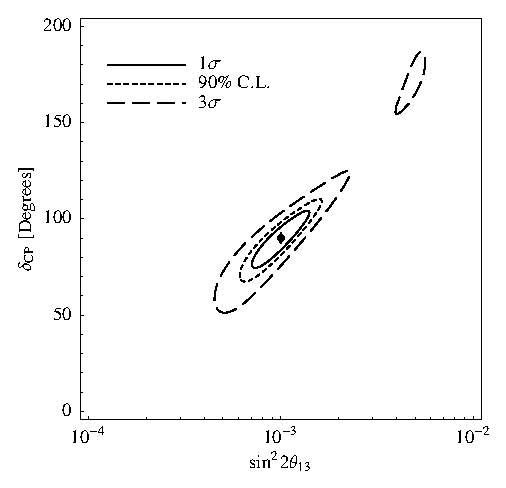
\includegraphics[width=7.7cm]{correx}}
\end{center}

}

Keeping all oscillation parameters and matter density scaling factors fixed,
 one can use the following builtin functions to obtain the total $\chi^2$ of all 
 specified oscillation channels including systematics:
\begin{function} 
\GLBNS{ChiSys}
{\tt double glbChiSys(const glb\_params in,int exp, int rule)} returns
the $\chi^2$ for the (fixed) oscillation parameters {\tt in}, the
experiment number {\tt exp}, and the rule number {\tt rule}. For all
experiments or rules, use \GLBC{GLB\_ALL} as parameter value.
\end{function}
Note that the result of {\tt glbChiSys} for all experiments or rules
corresponds to the sum of all of the individual {\tt glbChiSys} calls. 
This equality will not hold for the minimizers in the next chapters anymore. 
 An example how to use  {\tt glbChiSys} can be found on page~\pageref{ex:corrth13dcp}.  

\index{norm}{Systematics} \index{norm}{Pull method}
The treatment of systematics in \GLOBES\ is performed by the so-called
{\em pull method} with the help of nuisance systematics parameters.
They are taken to be completely uncorrelated among different rules,
and treated with simple Gau\ss ian statistics.
In general, a rule is a prescription for summing up experimentally indistinguishable
signal and background events from different oscillation channels.
For more details on the rule concept, see \Part~\ref{part:2} of this manual,
and for the treatment of systematics, see \Sec~\ref{sec:rules}.
 
 One example for a systematics parameter is the signal normalization error, \ie, an error on the overall normalization of the signal. For illustration, we assume that the signal event rate in the $i$th bin $s_i^0$ of one oscillation channel is altered by the overall normalization nuisance parameter\index{norm}{Nuisance parameter} of this channel, \ie , 
\be
 s_i = s_i(n_s) = s_i^0 \cdot (1 + n_s),
\ee
where $n_s$ is the signal normalization parameter. The total number of events in the $i$th bin $x_i$ also includes the background event rates $b_i$, \ie, $x_i = s_i + b_i$, which may have their own systematics parameters.
In order to implement an overall signal normalization error $\sigma_{n_s}$,  the $\chi^2$, which includes all event rates $x_i$ of all bins, is minimized over the nuisance parameter $n_s$:
\be
 \hat{\chi^2} = \underset{n_s}{\mathrm{min}} \left(  \chi^2(n_s, \hdots) + \frac{(n_s)^2}{\sigma_{n_s}^2} \right).
\ee 
This minimization is done independently for all nuisance parameters of the rule. The total $\chi^2$ for the considered experiment is finally obtained by repeating this procedure for all rules and adding their $\chi^2$-values. In general, the situation is more complicated because of the usage of many systematical errors. More details about systematics parameters and the definition of signal, background, and oscillation channels can be found in \Sec~\ref{sec:rules}, too.

The systematics minimization of an experiment can be easily switched on and off with \GLB{SwitchSystematics}, \ie, one can also compute the $\chi^2$ with statistics only. In addition, several options for 
systematics are available, such as only using total event rates without
spectral information. For details, we refer to \Chapt~\ref{chapt:running}.


\section{User-defined systematics calculation$^*$}
\index{norm}{Systematics!user-defined}
\label{sec:userchi}



\example{Systematics for a reactor setup with near and far detector}{\label{ex:syst}
\index{norm}{Systematics!Example, user-defined}

The following code fragment from the much more extensive {\tt example5.c}
calculates $\chi^2$ for a reactor setup with two detectors
including five different systematical errors: the flux normalization
of the reactor ({\tt x[0]}), the fiducial mass uncertainties of the far
({\tt x[1]}) and near ({\tt x[2]}) detector, and energy calibration errors for the far
({\tt x[3]}) and near ({\tt x[4]}) detectors.  The calculation follows
\equ{chi2reactor}, but includes the energy calibration.

\vspace*{-0.3cm}

\begin{quote}{\tt \footnotesize
double likelihood(double true\_rate, double fit\_rate, double sqr\_sigma) \\
\{ if (sqr\_sigma > 0) return square(true\_rate - fit\_rate) / sqr\_sigma; else return 0.0; \} 

double chiDCNorm(int exp, int rule, int np, double *x, double *errors, \\
  \hspace*{0.3cm}  void* user\_data) \\
\{ \\
  \hspace*{0.3cm} const EXP\_FAR = 0; const EXP\_NEAR = 1; \\
  \hspace*{0.3cm} int n\_bins = glbGetNumberOfBins(EXP\_FAR); \\
  \hspace*{0.3cm} double *true\_rates\_N = glbGetRuleRatePtr(EXP\_NEAR, 0); \\
  \hspace*{0.3cm} double *true\_rates\_F = glbGetRuleRatePtr(EXP\_FAR, 0); \\
  \hspace*{0.3cm} double signal\_fit\_rates\_N[n\_bins]; double signal\_fit\_rates\_F[n\_bins]; \\
  \hspace*{0.3cm} double signal\_norm\_N, signal\_norm\_F; \\
  \hspace*{0.3cm} int ew\_low, ew\_high, i; \\
  \hspace*{0.3cm} double emin, emax, fit\_rate;  double chi2 = 0.0; 

   \hspace*{0.3cm} /* Request simulated energy interval and analysis energy window */ \\
   \hspace*{0.3cm} glbGetEminEmax(exp, \&emin, \&emax); \\
   \hspace*{0.3cm} glbGetEnergyWindowBins(exp, rule, \&ew\_low, \&ew\_high); 

  \hspace*{0.3cm} /* Apply energy calibration error */ \\
  \hspace*{0.3cm} glbShiftEnergyScale(x[3], glbGetSignalFitRatePtr(EXP\_FAR, 0), \\
  \hspace*{0.9cm}                    signal\_fit\_rates\_F, n\_bins, emin, emax); \\
  \hspace*{0.3cm} glbShiftEnergyScale(x[4], glbGetSignalFitRatePtr(EXP\_NEAR, 0), \\
  \hspace*{0.9cm}                    signal\_fit\_rates\_N, n\_bins, emin, emax); 

  \hspace*{0.3cm} /* Loop over all bins in energy window */ \\
  \hspace*{0.3cm} signal\_norm\_F = 1.0 + x[0] + x[1]; \\
  \hspace*{0.3cm} signal\_norm\_N = 1.0 + x[0] + x[2]; \\
  \hspace*{0.3cm} for (i=ew\_low; i <= ew\_high; i++) \\
  \hspace*{0.3cm} \{ \\
  \hspace*{0.6cm}  /* Statistical part of chi2 for far detector */ \\
  \hspace*{0.6cm}  fit\_rate  = signal\_norm\_F * signal\_fit\_rates\_F[i]; \\
  \hspace*{0.6cm}  chi2 += likelihood(true\_rates\_F[i], fit\_rate, true\_rates\_F[i]); \\
   
  \hspace*{0.6cm}  /* Statistical part of chi2 for near detector  */ \\
  \hspace*{0.6cm}  fit\_rate  = signal\_norm\_N * signal\_fit\_rates\_N[i]; \\
  \hspace*{0.6cm}  chi2 += likelihood(true\_rates\_N[i], fit\_rate, true\_rates\_N[i]); \\
  \hspace*{0.3cm} \} 

  \hspace*{0.3cm} /* Systematical part of chi2 (= priors) */ \\
  \hspace*{0.3cm} for (i=0; i < np; i++)  chi2 += square(x[i]/errors[i]);

 \hspace*{0.3cm} return chi2; \\
\} 
}
\end{quote}
}

For some experimental setups, the built-in systematics functions are not sufficient
because they cannot handle systematical errors that are correlated between different
parts of a multi-detector setup. Therefore \GLOBES\ allows the user
to override the default $\chi^2$ calculation. The reader who wants to use this
feature should be familiar with \Secs~\ref{sec:event_rates},~\ref{sec:systematics},~\ref{sec:channel}, and~\ref{sec:rules}
of the manual. Note that this is an advanced topic, which requires \GLOBES\ 3.0 or
higher. It can be omitted in a first reading of the manuscript.

User-defined systematics is, compared to the built-in systematics, a compound between
the \AEDL\ definition and some source code defining the behavior. In the simplest case,
the \AEDL\ file defines user-defined systematics for a specific rule, gives it a 
name/identifier, and defines the systematical errors. The source code has then to match this \AEDL\
definition -- therefore, make sure to use only unique identifiers. 
Ones needs to register the user-defined systematics in the 
source code (typically after {\tt glbInit}) with
\begin{function}
\GLBNS{DefineChiFunction}
{\tt int glbDefineChiFunction(glb\_chi\_function chi\_func, int dim, const char *name, void* user\_data)}
 tells \GLOBES\ to register the user-defined systematics $\chi^2$ function {\tt chi\_func} 
identified by the string {\tt name} with {\tt dim} systematics parameters. The parameter {\tt user\_data}
is an arbitrary pointer being transferred to {\tt chi\_func}. It can, for instance, be used to avoid
global variables. Returns zero, if successful.
\end{function}
The user-defined systematics function itself has to have the pre-defined type 
\begin{function}
\GLBNS{\_chi\_function}
{\tt double (*glb\_chi\_function)(int exp, int rule, int dim, double *params, double *errors, void* user\_data)}.
In this function type, {\tt exp} is the experiment number, {\tt rule} is the rule number, {\tt dim} is the number of systematics parameters, {\tt params} is an array of the systematics nuisance parameters themselves, and {\tt errors} is an array with the systematical errors. The parameter {\tt user\_data} is set as defined with
{\tt glbDefineChiFunction}.
Note the the central values for {\tt params} are $0$, which means that $0$ corresponds to the un-modified rates. The array indices run from $0$ to {\tt dim}-1.
\end{function}
Note that this function will be called many times by the \GLOBES\ minimizers.
Therefore the function should be as efficient as possible.
%JK - THIS IS INCORRECT: ONE MINIMIZATION OVER, SAY, 8 PARAMETERS IS FASTER THAN
%2 MINIMIZATIONS OVER 4 PARAMETERS EACH-
%In many cases, it is also recommendable to use different functions for different
%rules, since the fewer auxiliary parameters in the minimization, the faster the routine will be.
In addition, note that complicated systematics with many parameters may introduce complicated (unknown) topologies for the minimization, which means that the minimizers may
end up in a local minimum instead of the global minimum. \GLOBES\ provides the function \GLB{SetSysStartingValuesList} to change the starting values of the minimizer in the case of
 convergence problems (see below).
A typical implementation may look like the following code, where ``{\tt chiDCNorm}'' is the identifier
assigned in the \AEDL\ definition:
\begin{quote}
{\tt
  double chiDCNorm(int exp, int rule, int dim, double *x, \\
  \hspace*{0.5cm} double *errors, void* user\_data) \\
  \{ \\
   \hspace*{0.5cm} double chi2 = 0.0; \\
   \hspace*{0.5cm} int i; \\
   \\
   \hspace*{0.5cm} ... /* Some code to calculate the chi2 */ \\
   \\
    \hspace*{0.5cm} /* Here the systematics priors (penalties) are added: */ \\
    \hspace*{0.5cm} for(i=0;i<dim;i++) chi2 += (x[i]*x[i])/(errors[i]*errors[i]);
    \hspace*{0.5cm} return chi2; \\
  \} \\
   \\
  int main(int argc,char*argv[]) \\
 \{ \\ 
  \hspace*{0.5cm} ... \\
  \hspace*{0.5cm} glbInit(agrv[0]); \\
  \hspace*{0.5cm} glbDefineChiFunction(\&chiDCNorm,5,"chiDCNorm",NULL); \\
  \hspace*{0.5cm} ... \\
 \} \\
}
\end{quote}

During running time, the systematics can be changed with 
\GLB{SetChiFunction} and \GLB{GetChiFunction} as described in \Sec~\ref{sec:systematics}.
In addition, especially useful in the context of user-defined systematics, a pointer to the systematics function can be returned either by name, or by experiment and rule selection:
\begin{function}
\GLBNS{GetChiFunctionPtr}
{\tt glb\_chi\_function glbGetChiFunctionPtr(const char *name)}
returns a pointer to the systematics $\chi^2$ function with a specified name {\tt name}.
\end{function}
\begin{function}
\GLBNS{GetChiFunctionPtrInExperiment}
{\tt glb\_chi\_function glbGetChiFunctionPtrInExperiment(int exp, int rule, int on\_off)}
returns a pointer to the systematics $\chi^2$ function of experiment {\tt exp} and rule {\tt rule}.
Systematics on or off can be accessed by {\tt on\_off}.
\end{function}

The user-defined $\chi^2$ function of type {\tt glb\_chi\_function} may use a number of helper functions for
for the $\chi^2$ calculation. 
A very useful function to include energy calibration errors is
\begin{function}
\GLBNS{ShiftEnergyScale}
{\tt glbShiftEnergyScale(double b, double *rates\_in, double *rates\_out,int bins, double emin, double emax)}
shifts the energy scale in {\tt rates\_in} by the relative amount {\tt b} and stores the result in 
{\tt rates\_out}. The parameters {\tt emin} and {\tt emax} denote the minimal and maximal energy
as obtained with \GLB{GetEminEmax}. Requires constant energy bin widths!
\end{function}
For details on energy calibration errors, see \Sec~\ref{sec:rules}.
%
In addition, in order to implement user-defined systematics, one usually needs low-level access to the event rate vectors using \GLB{GetRuleRatePtr}, \GLB{GetSignalFitRatePtr}, \GLB{GetBGFitRatePtr} and possibly other functions described in \Sec~\ref{sec:event_rates}. Additionally, the
functions \GLB{GetEminEmax}, \GLB{GetEnergyWindow}, \GLB{GetEnergyWindowBins}, and \GLB{GetNumberOfBins} from \Sec~\ref{sec:aedl_names} are useful.  We recommend that you familiarize yourself with these functions at this point.

Let us now discuss a simple example.  Typical applications for user-defined systematics are reactor neutrino experiments, where systematics play a crucial role. For a setup with near and far detectors,
the Gaussian formula for $\chi^2$ is
\begin{align}
  \chi^2 =& \sum_{i=1}^{\textrm{\# of bins}} \sum_{d = N,F} 
     \frac{\left( O_{d,i} - (1 + a_R + a_d) T_{d,i} \right)^2 }{O_{d,i}} + \frac{a_R^2}{\sigma_R^2} + \frac{a_N^2}{\sigma_N^2} + \frac{a_F^2}{\sigma_F^2}
\label{equ:chi2reactor}
\end{align}
% WAS POSSONIAN
% \begin{align}
%   \chi^2 =& \sum_{i=1}^{\textrm{\# of bins}} \sum_{d = N,F} 2
%      \left( O_{d,i} - (1 + a_R + a_d) T_{d,i} +
%        (1 + a_R + a_d) T_{d,i} \log \frac{(1 + a_R + a_d) T_{d,i}}{O_{d,i}}  \right) \nonumber\\
%          & \ \ + \frac{a_R^2}{\sigma_R^2} + \frac{a_N^2}{\sigma_N^2} + \frac{a_F^2}{\sigma_F^2}
% \label{equ:chi2reactor}
% \end{align}
where $O_{N,i}$ and $O_{F,i}$ are the event rates for the $i$-th bin in the near and
far detector, calculated for the assumed ``true'' values of the oscillation parameters.
$T_{d,i}$ are the event rates for the parameter values that are currently being tested.
$a_R$, $a_N$ and $a_F$ parameterize the small uncertainties in the reactor flux and the fiducial
mass of the two detectors. In this example, their central values are assumed to be zero,
while their standard deviations are $\sigma_R$, $\sigma_N$ and $\sigma_F$.
%
\begin{figure}[t]
\begin{center}
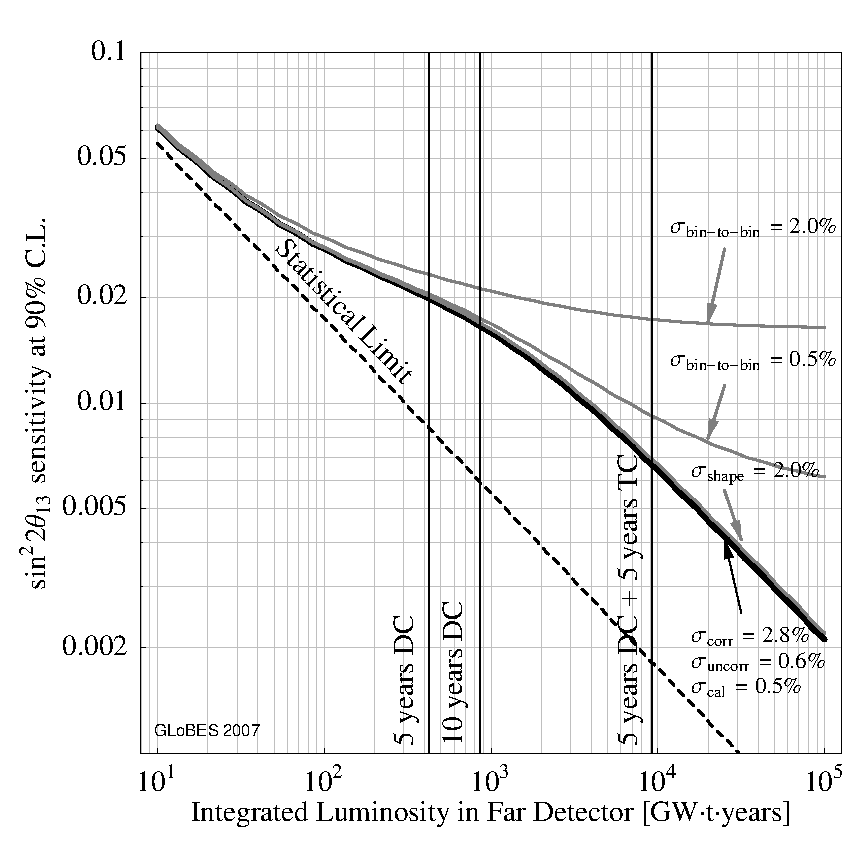
\includegraphics[width=10cm]{reactor}
\end{center}
\mycaption{\label{fig:reactor} The result from {\tt example5.c} (figure similar to the one
in \Ref~\cite{Huber:2006vr}). The thick curve corresponds to the systematics on page~\pageref{ex:syst}.}
\end{figure}
%
The first line of \equ{chi2reactor} is the standard $\chi^2$ expression for
the Gauss distribution, while the terms in the second line are penalties
for deviations of the systematics parameters from their central values. 
%
We use two \AEDL\ files for this experiment, one for the far detector and one for the
near detector.
The corresponding rule definition ($\nu_e$ disappearance) in the far detector \AEDL -file is
\begin{quote}
{\tt
rule(\#rule0)< \\
\hspace*{0.5cm}        @signal     = 1.0@\#nu\_e\_disappearance\_CC \\
\hspace*{0.5cm}        @background = 0.0@\#nu\_e\_disappearance\_CC   /* No background */ \\
\hspace*{0.5cm} @energy\_window = 0.0015 : 0.01 \\
\\
\hspace*{0.5cm}        @sys\_off\_function = "chiNoSysSpectrum" \\
\hspace*{0.5cm}        @sys\_off\_errors   = \{ \} \\
\hspace*{0.5cm}        @sys\_on\_function  = "chiDCNorm" \\
\hspace*{0.5cm}        @sys\_on\_errors    = \{ 0.028,    0.006,        0.006,       0.005,     0.005   \} \\
\hspace*{0.5cm}        \mbox{ // \{ Flux, Fid. mass FD, Fid. mass ND, Energy FD, Energy ND \} } \\
> 
}
\end{quote}
In this case, the systematics is called ``{\tt chiDCNorm}'' for systematics on, whereas systematics
off is computed with spectral information, but without systematical errors.
For the near detector \AEDL -file, we have instead
\begin{quote}
{\tt
rule(\#rule0)< \\
\hspace*{0.5cm}        @signal     = 1.0@\#nu\_e\_disappearance\_CC \\
\hspace*{0.5cm}        @background = 0.0@\#nu\_e\_disappearance\_CC   /* No background */ \\
\hspace*{0.5cm} @energy\_window = 0.0015 : 0.01 \\
\\
\hspace*{0.5cm}        @sys\_off\_function = "chiNoSysSpectrum" \\
\hspace*{0.5cm}        @sys\_off\_errors   = \{ \} \\
\hspace*{0.5cm}        @sys\_on\_function  = "chiZero" \\
\hspace*{0.5cm}        @sys\_on\_errors    = \{ \} \\
> 
}
\end{quote}
In this case, the systematics {\tt chiZero} is used for systematics on, which means that there will
be no active $\chi^2$ calculation in this rule. With this definition, the user-defined systematics
will only be called once for the far detector. However, the rates from the near detector will be 
passively provided for the common $\chi^2$ function.
You can find the corresponding files {\tt dchooz-near.glb} and {\tt dchooz-far.glb} you will need for {\tt example5.c}, in the example directory. 
%
We show the implementation of the $\chi^2$ function in the example on page~\pageref{ex:syst},
where we in addition include an uncorrelated energy calibration error. See \figu{reactor} for the result
of this example.
%

In cases where the systematics minimization does not converge fast enough or ends
up in a local minimum, one can change the starting values of the minimizer, \ie, the
starting point from which the local minimizer rolls into the local minimum.
\begin{function}
\GLBNS{SetSysStartingValuesList} 
{\tt int glbSetSysStartingValuesList(int exp, int rule, int on\_off, const double *sys\_list)}
sets the starting values of the local systematics minimizer in experiment {\tt exp} and 
rule {\tt rule} to the values in {\tt sys\_list}. This change can be performed for
systematics on or systematics off by using {\tt GLB\_ON} or {\tt GLB\_OFF} for {\tt on\_off}. 
Usually, zero is used for all starting values. 
\end{function}
\begin{function}
\GLBNS{GetSysStartingValuesListPtr} 
{\tt double *glbGetSysStartingValuesListPtr(int exp, int rule, int on\_off, const double *sys\_list)}
returns the starting values of the local systematics minimizer in experiment {\tt exp} and 
rule {\tt rule}. This list can be obtained for
systematics on or systematics off by using {\tt GLB\_ON} or {\tt GLB\_OFF} for {\tt on\_off}.
\end{function}
A useful trick is often to use the minimum from the last run as starting values for the next one
if the input parameters are only slightly changed. One can obtain the minimum from the last run 
from the last call of the $\chi^2$ function (\cf, {\tt example5.c}).


%%%%%%%%%%%%%%%%%%%%%%%%%%%%%%%%%%%%%%%%%%%%%%%%%%%%%%%%%%%%%%%%%%%%%%%%%%%%%%
\chapter[Calculating $\chi^2$-projections: how one can include correlations]{Calculating $\boldsymbol{\chi^2}$-projections: how one can include correlations}
\label{chapt:correlations}
\index{norm}{Correlation!and $\Delta\chi^2$}

This chapter deals with the rather complicated issue of $n$-parameter correlations. It is one of the greatest strengths of this software 
to include the full $n$-parameter correlation in the high-dimensional parameter space with reasonable effort. Of course, calculating $\chi^2$-projections is somewhat more complicated than using systematics only. Therefore, we use a simple step by step introduction to the problem. 

\index{norm}{Correlation!multi-parameter}


\section{Introduction}

\index{norm}{Projection!of manifold}
In principle, the precision of an individual parameter measurement including
 correlations in the $\chi^2$-approach can be obtained as the projection of 
the $n$-dimensional fit manifold onto the respective axis. Similarly, one can 
project the fit manifold onto a plane, such as the $\stheta$-$\deltacp$-plane,
 if one wants to show the allowed
region in this plane with all the other parameter correlations included. 
In practice, this projection (or marginalization) is very difficult: a grid-based method would 
need $(N_{\mathrm{grid}})^n$ function calls of {\tt glbChiSys} to 
calculate the projection onto one dimension 
including the full $n$-parameter correlation, where 
$N_{\mathrm{grid}}$ is the number of points in each direction of the 
lattice. For example, taking only $N_{\mathrm{grid}}=20$ and 
$n=7$ (six oscillation parameters and matter density) would mean more 
than one billion function calls of {\tt glbChiSys}. One can easily imagine 
that these would be too many for any reasonable application.

\index{norm}{Minimizer}
The solution to this problem is using a $n$-dimensional, local 
minimizer for the projection instead of a grid-based method, where we will
illustrate this minimization process later. It turns out
that such a minimizer can include a full $6$-parameter correlation 
with of the order of $1\, 000$ function calls of {\tt glbChiSys}. For the 
minimization we use a derivative free method due to Powell in a 
modified~\cite{Brent:1973} version\footnote{Not to need derivatives is
highly desired, since the event rate depends in a non-linear way on the
oscillation parameters. Thus, there is no easy analytical way
to obtain derivatives of the $\chi^2$ function.}.

Thus, for each point on the projection axis/plane, one can obtain a result within several seconds on a modern computer, which means that the complete measurement precision for one fixed true parameter set can be obtained in a few minutes. One can easily imagine that such a minimizer makes more sophisticated applications possible with the help of overnight calculations, such as showing the dependencies on the true parameter values.

This approach also has one major disadvantage: There is \emph{no} such
thing as a global minimization algorithm or even an algorithm which guarantees
to find \emph{all} local minima of a function. In practice this means using 
 a local minimizer, one may end up in an unwanted local minimum and not in 
the investigated (possibly global) one or 
one may miss a local minimum which affects the results\footnote{NB -- 
Implementing a grid-based method which guarantees to find all local minima is
not straightforward either, to say the least.}. 
The only way out of this dilemma is to use some heuristic approach, \ie , 
one can use schemes which work
in most cases and announce their failure loudly. In order to use such a
heuristic some (analytical or numerical) knowledge on the topology of 
the fit manifold is necessary. With this knowledge it is possible
to obtain an approximate position for each local minimum 
and thus to start the local minimizer 
close enough to the investigated minimum.
 Fortunately, this can be done quite straightforwardly in most cases, since 
the structure of the neutrino oscillation formulas does not cause very 
complicated topologies of the fit manifolds. Especially the simulation of 
reactor experiments and conventional beams or superbeams is rather simple 
with purely numerical
approaches. Neutrino factories have, especially for small values of
$\theta_{13}$, a much more complicated topology. In this case, results
of the many analytical discussions of this issue can be used. This means
 that one can implicitly use the analytical knowledge to obtain 
better predictions for the location of a minimum. One can easily imagine 
that the used methods then also depend
on the region of the parameter space. In this manual, we mainly use
examples with a neutrino factory, since some of these complications
can be illustrated there. Note that the methods described here are neither
complete, nor will they work everywhere in the parameter space. It is
in any case up to the user to make sure that the results are what he/she
thinks.

Some more words of warning with respect to results obtained by projecting
the $\chi^2$:
The results obtained this way are always only an \emph{upper} bound on the
value of the projected $\chi^2$ function, \ie\ an undiscovered minimum 
decreases the value of the the projected $\chi^2$ function. If the value
of the $\chi^2$ function in the missed minimum is larger than the
previously found ones it will not influence the value of the projected 
value. 
Thus, one can only run the danger to obtain a too optimistic solution 
if one does not find the other local minima appearing 
below the chosen confidence level. With this approach and proper usage,
 it should not be possible to produce a too pessimistic solution. 
However, if one is not careful enough to locate
all local minima, one can easily produce too optimistic solutions.
This danger can be summarized as follows:
\begin{equation}
\mathrm{Too \, pessimistic \, result} \, < \, \underbrace{\mathrm{Real \, result}}_{\mathrm{Located \, by \, careful \, usage}} \, \le \, \mathrm{\GLOBES \, result} \,  < \,  \mathrm{Too \, optimisitic \, result} \nonumber
\end{equation}

\index{norm}{External information!priors} 
\index{norm}{External information!input errors} 
\index{norm}{External information!central values}
In many cases, the fit manifold is restricted by the knowledge 
from earlier experiments. For example, the knowledge on the solar 
parameters will in most cases be supplied by the solar neutrino experiments. 
If, at the time of the measurement, the external precision of a parameter is
better than the one of the considered experiment itself, one usually will use
this better, external knowledge and impose a corresponding constraint
 on this parameter. The external knowledge may reduce the extension of the 
$n$-dimensional fit manifold in the respective direction. In the most 
extreme case, keeping all parameters but the measured one fixed 
in the analysis is equivalent to the assumption that all parameters 
are determined externally with infinitively high precision. As this 
is quite a strong assumption, one should \emph{always} check the 
consequences of relaxing it and using realistic errors. Only if such
a test has demonstrated that the impact of the uncertainty on a 
given fit parameter is negligible, it can safely be assumed as fixed. 
 The inclusion of external input in \GLOBES\ is done by the use of 
Gau\ss ian {\em priors}: We assume that an external measurement has 
determined the measured parameter to be at the \emph{central value}
with a $1 \sigma$ Gau\ss ian error (which we call {\em input error}).
The explicit definition of these priors will be shown in the next section. 

\section{The treatment of external input}
\label{sec:externalinput}

\index{norm}{External information}
\index{norm}{External input| \see{External information}}
It is one of the strengths of the \GLOBES\ software to use external input 
in order to reduce the extension of the fit manifold with the knowledge 
from external
(earlier) measurements. The treatment of external input is done by the 
addition of Gau\ss ian so-called {\em priors} to the systematics-minimized 
$\chi^2$-function. For example, for the matter density, one obtains as the 
final projected $\chi^2_F$ after minimization over the matter density
scaling factor \index{norm}{Matter density!scaling factor} $\hat{\rho}$
\be
 \chi^2_F = \underset{\rho}{\mathrm{min}} \left( \chi^2(\hat{\rho}) +
 \frac{(\hat{\rho} - \hat{\rho}^0)^2}{\sigma_{\hat{\rho}}^2} \right).
\label{equ:priors}
\ee
This example is a very simple one, since in fact the
minimization is simultaneously performed over all priors and free oscillation 
parameters. In \equ{priors}, $\hat{\rho}^0$ is the {\em central value} of the 
prior, and $\sigma_{\hat{\rho}}$ the $1 \sigma$ absolute (half width) 
{\em input error}. Thus, it is assumed that an external measurement has 
determined the matter density with a precision (input error) 
$\sigma_{\hat{\rho}}$ at the central value $\hat{\rho}^0$. Usually, 
the central value is fixed at the best-fit value, and the input error 
is chosen as the $1 \sigma$ half width of the external measurement. For the matter 
density, $\hat{\rho}^0$  is usually set to $1.0$, corresponding to
the actual matter density profile such as given by the experiment
 definition file, and $\sigma_{\hat{\rho}}$ to the 
relative matter density uncertainty (\eg, $0.05$ for 5\% uncertainty).

In principle, one can set the priors for the matter density and all oscillation parameters. For example, if the disappearance channels of the experiment determine the leading oscillation parameters with unprecedented
precisions, one can omit the respective input errors. In \GLOBES , an input error
value of $0$ corresponds\footnote{To be precise, a value for the error
in between $-10^{-12}$ and $+10^{-12}$} to neglecting the prior. If, however,
 earlier external measurements provide better information, one can set their 
absolute precisions with the input errors. The central values are usually 
chosen to be the best-fit values of this external experiments, such as
for the input from solar experiments. In some cases, it may be
necessary to adjust them, such as for artificial constraints to the
oscillation parameters. 
For example, for the investigation of the
opposite-sign solution, one can use the prior to constrain $\ldm$
in order to force the minimizer not to  fall into the (unwanted) 
true-sign solution. In this case, the central value of $\ldm$ would 
be set to $\rho^0_{\ldm} = - \ldm$, and a $\sigma_{\ldm}$ of the order 
of $\ldm$ would be imposed. For the algorithm, it would 
then be rather difficult 
to converge into the unwanted true-sign solution. However, note that 
one should in this case check that the actually determined value 
for $\ldm$ after minimization is close enough to the guessed value $-\ldm$ 
in order to avoid significant artifical contributions of the priors to the 
final $\chi^2$. Alternatively one could re-run the minimizer with the
position of the previously found minimum as starting position but now
with switching off the constraint on $\ldm$.

\index{norm}{External information!input errors} 
\index{norm}{External information!central values}
In order to set the central values and input errors, two function have to
 be called {\em before the usage of any minimizer}:
\begin{function}
\GLBNS{SetCentralValues}
{\tt int glbSetCentralValues(const glb\_params in)} sets the central values for all of the following minimizer calls to {\tt in}.
\end{function}
\begin{function}
\GLBNS{SetInputErrors}
{\tt int glbSetInputErrors(const glb\_params in)}
 sets the input errors for all of the following minimizer calls to {\tt in}.
 An input error of $0$ corresponds to not taking into account the
 respective prior.
\end{function}
Accordingly, there are functions to return the actually set central values
and input errors:
\begin{function}
\GLBNS{GetCentralValues}
{\tt int glbGetCentralValues(glb\_params out)} writes the currently
set central values to {\tt out}.
\end{function}
\begin{function}
\GLBNS{GetInputErrors}
{\tt int glbGetInputErrors(glb\_params out)}
 writes the currently set input errors to {\tt out}.
\end{function}
All functions take or return as many matter density parameters as there are initialized experiments. In addition, they return $-1$ if the operation
was not successful.

\index{norm}{External information!precision}
Eventually, a typical initialization of the external input with
$10\%$ external precisions for the solar 
parameters\footnote{In fact, accelerator-based long-baseline experiments 
are primarily sensitive to the product $\sin 2 \theta_{12} \cdot \sdm$, 
which means that these errors effectively add up to an error of this 
product of about $15\%$.}, 
and $5\%$ matter density uncertainties for all experiments looks like this:
\begin{quote}
{\tt
 glbDefineParams(input\_errors,theta12*0.1,0,0,0,sdm*0.1,0);\\  
 glbSetDensityParams(input\_errors,0.05,GLB\_ALL);\\
 glbSetCentralValues(true\_values);\\
 glbSetInputErrors(input\_errors);\\
}
\end{quote}
In this example, the central values are set to 
the true (simulated) values.

%JK - NO LONGER TRUE IN GLOBES 3.0
%Remember that initially the 
%matter density scaling factors are 
%all $1.0$, which means that they do not need to be adjusted for the
%central values.

\index{norm}{Minimizer!priors}
\index{norm}{External information!priors}
\index{norm}{Advanced tricks}
Though the priors are an elegant way to treat external input, 
there are also some complications with priors. The following hints are for the
more advanced \GLOBES\ user:
\begin{enumerate}
\item
 The priors are only added once to the final $\chi^2$, no matter how
 many experiments there are simulated. This is already one reason
 (besides the minimization) why the sum of all projected $\chi^2$'s of 
 the individual experiments 
 cannot correspond to the $\chi^2$ of the combination of all experiments.
\item
 Priors are not used for parameters which are not minimized over, \ie, 
 kept fixed. This will be important together with arbitrary projections
 using \GLB{ChiNP}. A more subtle consequence is the comparison
 of fit manifold sections and projections for the solutions where
 the absolute minimum $\chi^2$ is larger than zero, \ie, degeneracies
 other than the true solution. In this case, the sections and
 projections are not  comparable if not corrected by the prior contributions, where the
 correction can be obtained as the $\chi^2$-difference at the minimum.
 For example, projecting the $\mathrm{sgn}(\ldm)$-degeneracy onto
 the $\theta_{13}$-$\deltacp$-plane and comparing it with the section
 (all other parameters fixed), the section region would in many cases be 
 larger than the projection region if the priors were not added to the
 section. At the true solution, this problem usually does not occur
 because the prior contributions are close to zero.    
\item
Currently, \GLOBES\ only supports Gau\ss ian pre-defined priors for the individual
oscillation parameters. Especially for the solar parameters, this is only
 an approximation, since they are imposed on $\theta_{12}$ and not
 on $\ldm$ or $\sin^2  \theta_{12}$. \GLOBES\ 3.0 and higher provide an alternative
to that by the concept of user-defined priors (\cf, \Sec~\ref{sec:userdefined}).
 \end{enumerate}

 
 
\example{Projection of two- and $n$-dimensional manifold onto $\stheta$-axis}{
\label{ex:corrproj}
\index{norm}{Projection!of manifold}
\index{norm}{Correlation!two-parameter}
\index{norm}{Correlation!multi-parameter}

This example demonstrates how to project the fit manifold onto the $\stheta$-axis, \ie, how one can include correlations. We compute two sets of data: one for keeping all parameters but $\deltacp$ fixed (two-parameter correlation), and one for keeping all parameters free (multi-parameter correlation). However, we impose external precisions for the solar parameters and the matter density. The following code excerpt is from 
{\tt example2.c}:

\begin{quote}
{\tt {\scriptsize
  /* Set central values and input errors for all projections */  \\
  glbDefineParams(input\_errors,theta12*0.1,0,0,0,sdm*0.1,0);\\  
  glbSetDensityParams(input\_errors,0.05,GLB\_ALL);\\
  glbSetCentralValues(true\_values);
  glbSetInputErrors(input\_errors);\\
\\
  /* Define my own two-parameter projection for glbChiNP: Only deltacp is free! */ \\
  glbDefineProjection(th13\_projection,GLB\_FIXED,GLB\_FIXED,GLB\_FIXED,GLB\_FREE,GLB\_FIXED,GLB\_FIXED); \\
 % HAS TO BE GLB_FIXED HERE; OTHEREWISE FIG. 4.1 DOES NOT MAKE SENSE!
  glbSetDensityProjectionFlag(th13\_projection,GLB\_FIXED,GLB\_ALL); \\
  glbSetProjection(th13\_projection); \\ 
\\
  /* Iteration over all values to be computed */ \\
  double x,res1,res2;     \\
  for(x=-4;x<-2.0+0.001;x=x+2.0/50) \\
  \{ \\
\hspace*{0.5cm}  /* Set fit value of stheta */ \\
\hspace*{0.5cm} glbSetOscParams(test\_values,asin(sqrt(pow(10,x)))/2,1); \\
    \\
\hspace*{0.5cm} /* Guess fit value for deltacp in order to safely find minimum */ \\
\hspace*{0.5cm} glbSetOscParams(test\_values,200.0/2*(x+4)*M\_PI/180,3); \\
 \\
\hspace*{0.5cm} /* Compute Chi2 for user-defined two-parameter correlation */ \\
\hspace*{0.5cm} res1=glbChiNP(test\_values,NULL,GLB\_ALL); \\
      \\
\hspace*{0.5cm} /* Compute Chi2 for full correlation: minimize over all but theta13 */ \\
\hspace*{0.5cm} res2=glbChiTheta13(test\_values,NULL,GLB\_ALL); \\
  \\
\hspace*{0.5cm} AddToOutput(x,res1,res2);\\
  \} 

}}
\end{quote}
The two lists of data then represent the $\stheta$ precisions with two-parameter correlations (gray-shaded) and multi-parameter correlations (arrows):
\begin{center}
\colorbox{white}{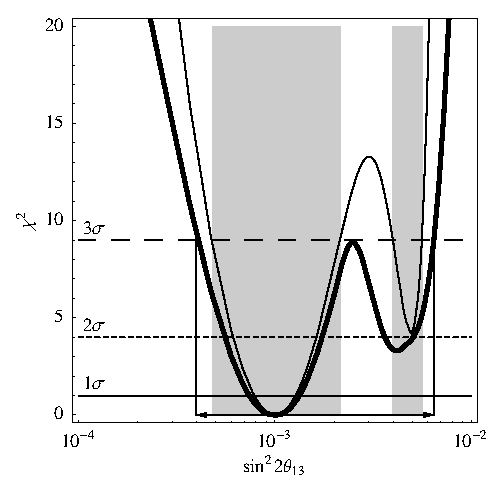
\includegraphics[width=6cm]{projallex}}

\vspace*{0.1cm}

\footnotesize{(Same parameters as on page~\pageref{ex:corrth13dcp} and in \figu{projex}, but 1 d.o.f.)}
\end{center}
}
%%%%%%%%%%%%%%%%%%%%%%%%%%%%%%%%%%%%%%%%%%%%%%%%%%%%%%%%%%%%%%%%%%%%%%%%
\section[Projection onto the $\stheta$-axis or $\deltacp$-axis]{Projection onto the $\boldsymbol{\stheta}$- or $\boldsymbol{\deltacp}$-axis}
\index{norm}{Projection!axis}

\begin{figure}[t]
\begin{center}
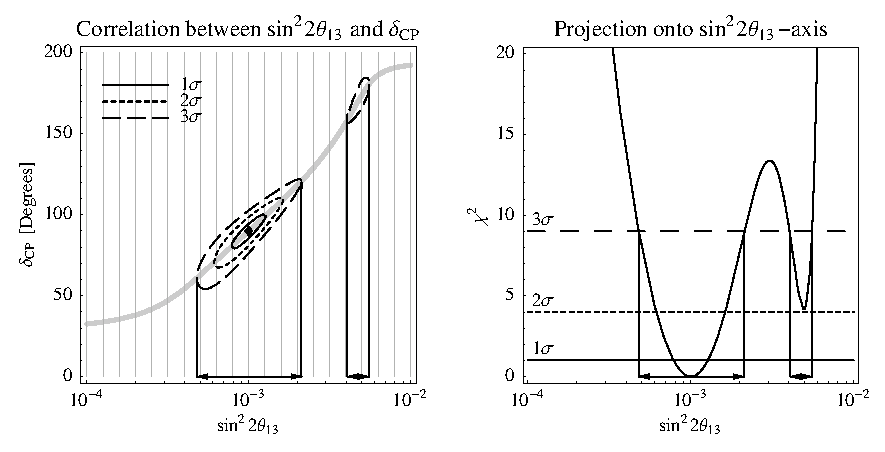
\includegraphics[width=16cm]{projex}
\end{center}
\mycaption{\label{fig:projex} Left plot: The correlation between $\stheta$ and $\deltacp$ as calculated in the example on page~\pageref{ex:corrth13dcp}, but for 1 d.o.f. only. Right plot: The $\chi^2$-value of the projection onto the $\stheta$-axis as function of $\stheta$. The projection onto the  $\stheta$-axis is obtained by finding the minimum $\chi^2$-value for each fixed value of $\stheta$ in the left-hand plot, \ie, along the gray vertical lines. The thick gray curve marks the position of these minima in the left-hand plot. The arrows mark the obtained fit ranges for $\stheta$ at the $3 \sigma$ confidence level (1 d.o.f.), \ie , the precision of $\stheta$.}
\end{figure}

The projection onto the $\stheta$- (or $\deltacp$-) axis is performed by fixing $\stheta$ (or $\deltacp$) and minimizing the $\chi^2$-function over all free fit parameters and the matter densities. We illustrate this method by the example of the projection of the two-dimensional manifold in the $\stheta$-$\deltacp$-plane onto the $\stheta$-axis in \figu{projex}. In this figure, the left-hand plot shows the correlation in the $\stheta$-$\deltacp$-plane computed with {\tt glbChiSys}. The right-hand plot illustrates the projection of this two-dimensional manifold onto the $\stheta$ axis by minimizing $\chi^2$ over $\deltacp$. In this simple example, the minimization is done along the vertical gray lines in the left hand plot. The obtained minima are located on the thick gray curve, which means that the right-hand plot represents the $\chi^2$-value along this curve. In fact, one can easily see that one obtains the correct projected $3 \sigma$ errors in this example (\cf, arrows). This figure illustrates the projection of a two-parameter correlation. In general, the full $n$-parameter correlation is treated similarly by the simultaneous (local) minimization over all free fit parameters. 

\index{norm}{Minimizer}
The following functions are some of the simplest minimizers 
provided by \GLOBES :
\begin{function}
\GLBNS{ChiTheta13}
{\tt double glbChiTheta13(const glb\_params in, glb\_params out, int exp)}
returns the projected $\chi^2$ onto the $\theta_{13}$-axis for the  experiment {\tt exp}. For the simulation of all initialized experiments,
use {\tt GLB\_ALL} for {\tt exp}. The values in {\tt in} are the guessed fit values for the minimizer (all parameters other than $\theta_{13}$) and the fixed fit value of $\theta_{13}$. The actually determined parameters at the minimum are returned in {\tt out}, where $\theta_{13}$ is still at
its fixed value. If {\tt out} is set to {\tt NULL}, this information will not be returned.
\end{function}
\begin{function}
\GLBNS{ChiDelta}
{\tt double glbChiDelta(const glb\_params in, glb\_params out, int exp)}
returns the projected $\chi^2$ onto the $\deltacp$-axis for the  experiment {\tt exp}. For the simulation of all initialized experiments,
use {\tt GLB\_ALL} for {\tt exp}. The values in {\tt in} are the guessed fit values for the minimizer (all parameters other than $\deltacp$) and the fixed fit value of $\deltacp$. The actually determined parameters at the minimum are returned in {\tt out}, where $\deltacp$ is still at its fixed value. If {\tt out} is set to {\tt NULL}, this information will not be returned.
\end{function}

All of the minimization functions have a similar parameter structure: The fixed fit parameter value and the guessed starting point of the minimizer, \ie, the guessed position of the minimum, are transferred in the list {\tt in}. Part of this list are the matter density
scaling factors of all experiments, which are also minimized over. 
The minimizer is then started at the guessed point and runs into
the local minimum, where the fit parameter of the projection
axis is fixed. For the true solution, it is usually sufficient to start 
the minimizer at the true parameter values. However, the convergence 
speed might
be better by starting it slightly off this point. In addition, there
are problems in many cases with more complicated topologies, which means
that better guesses for the position of the minimum are needed.
The position of the minimum is then returned in {\tt out}
together with the number of iterations used for the minimization.
It is very often useful to print the output of the minimization with
\GLB{PrintParams} in order to check that the minimum is the
appropriate one. For example, if the minimizer ends up in the wrong-sign
solution in $\ldm$, priors can be used to force it into the tested
minimum. In addition, the number of iterations used allows an optimization
of the convergence speed. 
% 
Note that before any minimization, \GLB{SetCentralValues} 
and \GLB{SetInputErrors} have to be used at least once. In addition, note that the resulting $\chi^2$ of {\tt glbChiTheta13} (or {\tt glbChiDelta}) for the combination of more than one experiment is not 
equal to the sum of the individual $\chi^2$-values anymore. This has two reasons: First, the topology of the fit manifold is altered by the addition of $\chi^2$-values of different experiments. Thus, after the minimization, the position of the minimum can be different to the ones of the individual experiments. Second, the priors for the external knowledge on the parameters are only added once -- independent of the number of experiments.

\index{norm}{Matter density!scaling factor}
The output of the minimizer in {\tt out} carries as many matter density scaling factors as there are experiments. Either
one (for the simulation of one experiment) or all (for the simulation of
all experiments) are different from $1.0$ if matter density uncertainties
are present, since each experiment may face other matter density conditions. 
The minimizers of individual experiments ``know'' which
experiment they are currently treating, which means that they only return the
matter density scaling factor of the appropriate experiment.
For example, calculating {\tt glbChiTheta13} for the last experiment
number, the last density value will be returned.
This approach turns out to be extremely useful together with the
simulation of more than one experiment. One can, for instance, locate the
degeneracies of all individual experiments. In order to test if
these degeneracies are still present in the combination of all experiments (which has a very different topology), one can test the combination of experiments with the output {\tt out} from the individual experiments. In this case, even the correct matter density scaling factor
output is used. 

The example on page~\pageref{ex:corrproj} demonstrates how one can obtain \figu{projex} (right) with keeping all parameters but $\deltacp$ fixed, as well as how one can include the full $n$-parameter correlation with external input. It also demonstrates how these two compare to each other. One can easily read off this example that 
there is a substantial impact of the
correlation with oscillation parameters other than $\deltacp$. 
Note that it uses the function
\GLB{ChiNP} for arbitrary projections from the next section for the minimization over $\deltacp$.
In addition, there is one interesting feature in guessing the
oscillation parameters in this example: In order to avoid falling
into the wrong minimum, the fit value of $\deltacp$ is guessed from \figu{projex} (left). This quite sophisticated ``guessing'' is typical
for neutrino factories because of the $(\deltacp, \theta_{13})$-degeneracy, whereas it is for superbeams often sufficient
to use the true values. A strong indication for a wrong guessing 
are discontinuous jumps in the projected $\chi^2$-function, where the minimizer jumps from one minimum to another. In such cases, the starting point of the minimizer has to be adjusted to help it find the true minimum.
%
Other examples for projections onto a parameter axis while keeping exactly one parameter fixed are \GLB{ChiTheta23}, \GLB{ChiDm31}, and \GLB{ChiDm21}, which
can be found in \Tab~\ref{tab:stdfunctions} on page~\pageref{tab:stdfunctions}.

Since the number of different parameter vectors used by \GLOBES\ may be a bit confusing, we summarize the most common parameter sets used in the calculations:
\begin{description}
\item[The simulated/true values] are the values set in \GLB{SetRates}.
\item[The fit values] are the values in the first parameter {\tt in} of {\tt glbChiTheta13} (and the other minimization functions) which are {\em fixed} by definition (such as $\theta_{13}$ for {\tt glbChiTheta13}). 
\item[The starting point/educated guess for the minimizer] are the values in the first parameter {\tt in} of {\tt glbChiTheta13} (and the other minimization functions) which are {\em free} by definition (such as all but $\theta_{13}$ for {\tt glbChiTheta13}). 
\item[The minimization result] of the marginalization process are the values in the second parameter {\tt out} of {\tt glbChiTheta13} (and the other minimization functions) which are {\em free} by definition (such as all but $\theta_{13}$ for {\tt glbChiTheta13}). The other values in {\tt out} still correspond to the fit values. 
\item[The position of external priors,] \ie, the best-fit values of external input, is set by \GLB{SetCentralValues}.
\item[The magnitude of external errors,] \ie, the errors of external input, is set by \GLB{SetInputErrors}.
\end{description}


%%%%%%%%%%%%%%%%%%%%%%%%%%%%%%%%%%%%%%%%%%%%%%%%%%%%%%%%%%%%%%
\section[Projection onto any hyperplane$^*$]{Projection onto any hyperplane$^*$}
\index{norm}{Projection!hyperplane}

In general, one can show the measurement result in any $k$-dimensional hyperplane, where $k$ is smaller than the dimension of the parameter space $n$, and thus the dimension of the fit manifold. In this case, $k$ parameters are fixed and $n-k$ parameters are minimized over. One such example is the projection of the fit manifold onto the $\stheta$-$\deltacp$-plane, \ie, $k=2$ here. In this case, the two
parameters $\stheta$ and $\deltacp$ are kept fixed, and the others are
minimized over. 
The corresponding function is 
\index{norm}{Projection!$\theta_{13}$-$\deltacp$-plane}
\begin{function}
\GLBNS{ChiTheta13Delta}
{\tt double glbChiTheta13Delta(const glb\_params in, glb\_params out, int exp)} returns the projected $\chi^2$ onto the $\theta_{13}$-$\deltacp$-plane for the  experiment {\tt exp}. For the simulation of all initialized experiments,
use {\tt GLB\_ALL} for {\tt exp}. The values in {\tt in} are the guessed fit values for the minimizer (all parameters other than $\theta_{13}$ and $\deltacp$) and the fixed fit values of $\theta_{13}$ and $\deltacp$. The actually determined parameters at the minimum are returned in {\tt out}, where $\theta_{13}$ and $\deltacp$ are still at their fixed values. If {\tt out} is set to {\tt NULL}, this information will not be returned.
\end{function}
This function works analogously to the ones in the last section. It can, for example, be used to obtain a figure similar to \figu{projex}, left, but with all other parameters marginalized over.
The example on page~\pageref{ex:corrproj} illustrates then the result of the
projection of the ``eggs'' within the 
$\stheta$-$\deltacp$-plane onto the $\theta_{13}$-axis. 
Though the running time for one call of these functions is somewhat 
shorter than the one for the $\stheta$- or $\deltacp$-projections, one 
has to compute a two-dimensional array for such a figure (instead of a 
one-dimensional list). Therefore, the overall computational effort is 
much higher, \ie, in the order of hours. In many cases, it is therefore
convenient to run {\tt glbChiSys} first to obtain a picture of
the manifold and to adjust the parameter ranges. Then, one can run
{\tt glbChiTheta13Delta} for a complete evaluation of the problem
including correlations.

\begin{table}[t!]
\begin{tabular}{p{4.2cm}p{5.5cm}p{5.1cm}}
\hline
Function & Purpose & Parameters $\rightarrow$ Result\\
\hline
\GLB{AllocProjection} & Allocate projection vector & {\tt ()} \\
\GLB{FreeProjection} & Free projection vector {\tt stale} & {\tt (glb\_projection stale)} \\
\GLB{DefineProjection} & Assign projection vector {\tt in} & {\tt (glb\_projection in, int theta12, int theta13, int theta23, int delta, int dms, int dma)} \\ 
\GLB{CopyProjection} & Copy vector {\tt source} to {\tt dest} & {\tt (const glb\_projection source, glb\_projection dest)} \\
\GLB{PrintProjection} & Print vector {\tt in} to file {\tt stream} & {\tt (FILE* stream, const glb\_projection in)} \\
\GLB{SetProjectionFlag} & Set flag for oscillation parameter {\tt which} in vector {\tt in} to value {\tt flag}. & {\tt (glb\_projection in, int flag, int which)} \\
\GLB{GetProjectionFlag} & Return flag for oscillation parameter {\tt which} in vector {\tt in}. & {\tt (const glb\_projection in, int which)} $\rightarrow$ {\tt int} flag \\
 {\tt glbSetDensity\-ProjectionFlag} \GLBNS{SetDensityProjectionFlag} & Set flag for density parameter {\tt which} in vector {\tt in} to value {\tt flag}. & {\tt (glb\_projection in, int flag, int which)} \\
{\tt glbGetDensity\-ProjectionFlag} \GLBNS{GetDensityProjectionFlag} & Return flag for density parameter {\tt which} in vector {\tt in}.  & {\tt (const glb\_projection in, int which)} $\rightarrow$ {\tt int} flag \\
\hline
\end{tabular}
\mycaption{\label{tab:defprojection}\index{norm}{Projection!type}
Different functions handling the
\GLB{\_projection} type. Flags are either \GLBC{GLB\_FIXED} or \GLBC{GLB\_FREE}. The (un-shown) return values of the {\tt Set-} and {\tt Define-} functions point either to the assigned vector if successful, or they are {\tt NULL} if unsuccessful.}
\end{table}

In principle, one can also use three- or more-dimensional projections. In addition, one may want to use a different set of parameters for single- or two-parameter projections. The very flexible function \GLB{ChiNP} is
designed for this purpose. However, because of its flexibility, it 
involves more sophistication.

In order to define arbitrary projections, we introduce the vector
\GLB{\_projection}, which is very similar to the
oscillation parameter vector {\tt glb\_params}.
Normally, the user does not need to access this type directly:
A set of function similar to the ones for {\tt glb\_params} is
provided. The purpose of {\tt glb\_projection} is to tell \GLOBES\ 
which parameters are fixed, and which are minimized over. Thus, in
comparison to {\tt glb\_params}, it does not take values for the
parameters, but flags \GLBC{GLB\_FIXED} or \GLBC{GLB\_FREE}.
For example, the projection onto the $\theta_{13}$-axis {\tt glbChiTheta13}
is nothing else than a special case of {\tt glbChiNP} with $\theta_{13}$
fixed and all the other parameters free. Similar to {\tt glb\_params},
the type {\tt glb\_projection} has to be allocated first, and freed
later. The access functions for {\tt glb\_projection} are summarized in \Tab~\ref{tab:defprojection}. Since the complete set is very similar to
the one for {\tt glb\_params}, we do not go into greater details here.

\index{norm}{Projection! definition}
As soon as we have defined a projection, we can assign it:
\begin{function}
\GLBNS{SetProjection}
{\tt int glbSetProjection(const glb\_projection in)} sets the projection
to {\tt in}. The return value is $0$ if successful, and $-1$ if
unsuccessful.
\end{function}
Similarly, the currently assigned projection can be returned with:
\begin{function}
\GLBNS{GetProjection}
{\tt int glbGetProjection(glb\_projection out)} writes the currently
set projection to {\tt out}. The return value is $0$ if successful, and $-1$ if unsuccessful.
\end{function}
After setting the central values, input errors, and the projection, 
we can run the minimizer:
\begin{function}
\GLBNS{ChiNP}
{\tt double glbChiNP(const glb\_params in, glb\_params out, int exp)} 
returns the projected $\chi^2$ onto the hyperplane specified by 
{\tt glbSetProjection} for the  experiment {\tt exp}. 
For the simulation of all initialized experiments,
use {\tt GLB\_ALL} for {\tt exp}. The values in {\tt in} are the guessed fit values for the minimizer (all free parameters) and the fit values
on the hyperplane (all fixed parameters). The actually determined parameters at the minimum are returned in {\tt out}, where the fixed parameters are still at their input values. If {\tt out} is set to {\tt NULL}, this information will not be returned.
\end{function}
As an example, the projection sequence for a minimization over
$\deltacp$ only (and the matter density parameters) looks like this:
\begin{quote}
{\tt
  glb\_projection th13\_projection = glbAllocProjection(); \\
  glbDefineProjection(th13\_projection,GLB\_FIXED,GLB\_FIXED,GLB\_FIXED,\\
  \hspace*{2cm} GLB\_FREE,GLB\_FIXED,GLB\_FIXED); \\
  glbSetDensityProjectionFlag(t13\_projection,GLB\_FIXED,GLB\_ALL); \\
  glbSetProjection(th13\_projection); \\ 
  res1=glbChiNP(test\_values,NULL,GLB\_ALL); \\
  glbFreeProjection(th13\_projection);
}
\end{quote}
In this case, only the correlation with $\deltacp$ is taken into account.
Note that in the  example on page~\pageref{ex:corrproj} this projection
is compared with the result including the full multi-parameter correlation.

%%%%%%%%%%%%%%%%%%%%%%%%%%%%%%%%%%%%%%%%%%%%%%%%%%%%%%%%%%%%%%
\section{User-defined priors$^*$}
\index{norm}{User-defined priors}
\label{sec:userdefined}

\example{Non-Gaussian external solar input}{
\label{ex:userprior}

This examples demonstrates how to use a non-Gaussian error for the
external solar mixing angle input instead of a Gaussian error.
The user-defined prior function reads as follows and is very similar to the standard prior:
\begin{quote}
{\tt {\footnotesize
 double my\_prior(const glb\_params in, void* user\_data) \\
\{ \\
  \hspace*{0.5cm} glb\_params central\_values = glbAllocParams(); \\
  \hspace*{0.5cm} glb\_params input\_errors = glbAllocParams(); \\
  \hspace*{0.5cm}  glb\_projection p = glbAllocProjection(); \\
  \hspace*{0.5cm}  glbGetCentralValues(central\_values); \\
  \hspace*{0.5cm}  glbGetInputErrors(input\_errors); \\
  \hspace*{0.5cm}  glbGetProjection(p); \\
  \hspace*{0.5cm}  int i; \\
  \hspace*{0.5cm}  double pv = 0.0; \\
  \hspace*{0.5cm}  double fitvalue,centralvalue,inputerror; 

 \hspace*{0.5cm} /* Add oscillation parameter priors */ \\
  \hspace*{0.5cm}  for(i=0;i<6;i++) \\
  \hspace*{0.5cm} if(glbGetProjectionFlag(p,i)==GLB\_FREE) \\
  \hspace*{0.5cm} \{ \\
  \hspace*{1cm} fitvalue=glbGetOscParams(in,i); \\
  \hspace*{1cm} centralvalue=glbGetOscParams(central\_values,i); \\
  \hspace*{1cm} inputerror=glbGetOscParams(input\_errors,i); \\
  \hspace*{1cm} if(inputerror>1e-12) 
  \hspace*{1cm} \{ \\
  \hspace*{1.5cm} if(i==GLB\_THETA\_12) /* Prior on $\sin^2 \theta_{12}$ */ \\ 
\hspace*{2.0cm} pv+=square((startvalue-square(sin(fitvalue)))/inputerror);\\ 
  \hspace*{1.5cm} else \\ 
  \hspace*{2.0cm}  pv+=square((startvalue-fitvalue)/inputerror); \\
  \hspace*{1cm} \} \\
  \hspace*{0.5cm} \} 

\hspace*{0.5cm} /* Add matter parameter priors */ \\
  \hspace*{0.5cm} for(i=0;i<glb\_num\_of\_exps;i++) \\
  \hspace*{0.5cm} if(glbGetDensityProjectionFlag(p,i)==GLB\_FREE) \\
  \hspace*{0.5cm} \{ \\
  \hspace*{1cm}  fitvalue=glbGetDensityParams(in,i); \\
  \hspace*{1cm}  centralvalue=1.0; \\
  \hspace*{1cm}  inputerror=glbGetDensityParams(input\_errors,i); \\
  \hspace*{1cm}  if(inputerror>1e-12) \\
  \hspace*{1.5cm}   pv+=square((centralvalue-fitvalue)/inputerror); \\
  \hspace*{0.5cm} \} 

  \hspace*{0.5cm} glbFreeParams(central\_values); \\
  \hspace*{0.5cm} glbFreeParams(input\_errors); \\
  \hspace*{0.5cm} glbFreeProjection(p); \\
  \hspace*{0.5cm} return pv; \\
\}
}
}

Note that this prior interprets the central values and input errors in terms of  $\sin^2 \theta_{12}$
instead of $\theta_{12}$.
\end{quote}
}

User-defined priors are an advanced concept of \GLOBES\ 3.0 and higher. Therefore,
this section can be skipped in a first reading of the manual.
They allow for arbitrary priors which depend on the oscillation parameters only (as opposed
to systematics; \cf, \equ{priors}).
Therefore, compared to user-defined systematics, they depend on the oscillation
parameters only, but not on the systematics parameters. Examples for applications
are non-Gaussian external input, the combination with externally simulated experiments, and the
constraint to certain parameter-subspaces (such as a specific octant).

The following function replaces the standard priors by user defined ones and has to be used
after {\tt glbInit}:
\begin{function}
\GLBNS{RegisterPriorFunction}
{\tt 
glbRegisterPriorFunction(double (*prior)(const glb\_params, void *user\_data), int (*central)(const glb\_params, void *user\_data), int (*error)(const glb\_params, void *user\_data),  void *user\_data)} registers a user-defined prior function {\tt prior}. In addition, it is possible to register
two functions {\tt central} and {\tt error} being called every time \GLB{SetCentralValues} or \GLB{SetInputErrors} are called with the same argument. For example, the central values and input errors can be stored in
global variables for a faster access. These pointers can also be {\tt NULL}. The pointer {\tt user\_data} can be optionally used to circumvent the use of global variables. It is set by {\tt glbRegisterPriorFunction} and transferred to the registered functions whenever called.
\end{function}

The prior function should expect the parameter structure {\tt glb\_params} containing the
current fit values and the {\tt void}-pointer {\tt user\_data} as arguments.
We show an example for a user-defined prior on page~\pageref{ex:userprior}. This prior
is simply registered with
\begin{quote}
{\tt
 glbInit(argv[0]); \\
 glbRegisterPriorFunction(my\_prior,NULL,NULL,NULL);
}
\end{quote}
and replaces the standard prior of \GLOBES . It behaves exactly as the standard prior, but
the solar mixing angle is interpreted as $\sin^2 \theta_{12}$ instead of $\theta_{12}$. Therefore,
a Gaussian error is imposed on $\sin^2 \theta_{12}$ instead of $\theta_{12}$, and the central
values and input errors are interpreted in terms of $\sin^2 \theta_{12}$ as well. Note that
one does not need to know if the prior was called for one experiment only or all experiments,
since this information is implicitly given by the different density projection flags being set
accordingly. 

%%%%%%%%%%%%%%%%%%%%%%%%%%%%%%%%%%%%%%%%%%%%%%%%%%%%%%%%%%%%%%%%%%%%%%%%%%%
\chapter{Locating degenerate solutions}
\index{norm}{Degeneracies|(}
\index{norm}{Degeneracies!multiple solutions}
\index{norm}{Degeneracies!and $\Delta\chi^2$}

Here we describe how one can locate degenerate solutions in \GLOBES , and we discuss
several techniques for the application software.

\section{Minimization over all oscillation parameters}

In the last chapter, we introduced marginalizations over different parameters to obtain measurement precisions. Similarly, one can minimize over {\em all} $n$ parameters to find the local minimum close to any starting point. This approach is very useful for the exact numerical location of a degeneracy if its approximate position is known. For the determination of the approximate position, one can use analytical approaches or an educated guess. 
Though the usage of the all-parameter minimizers is quite simple, one should keep in mind that they are local minimizers. Therefore, one may need a very sophisticated application software to find all degenerate solutions.

\example{Finding the $\mathrm{sgn}(\ldm)$-degeneracy}{
\label{ex:sgndeg}
\index{norm}{Degeneracies!sgn($\ldm$)-degeneracy}
\index{norm}{Mass hierarchy}

In many cases, one can find the exact position of the 
$\mathrm{sgn}(\ldm)$-degeneracy with \GLB{ChiAll}, where one starts 
the local minimizer at the suspected position 
and lets it run into the minimum.  The following code excerpt  corresponds to finding the degenerate solution for the example on
  page~\pageref{ex:corrth13dcp}, and it is from {\tt example3.c}: 
\begin{quote}
{\tt
{\footnotesize
  /* Set starting vales to suspected position at opposite sign of ldm */ \\
  \mbox{glbDefineParams(central\_values,theta12,theta13,theta23,deltacp,sdm,-ldm);} \\
  glbSetDensityParams(central\_values,1.0,GLB\_ALL); \\
  \\
  /* Set input errors for external input, where some information on ldm \\
   \hspace*{0.5cm} is imposed in order to avoid falling into the right-sign solution */ \\
  glbDefineParams(input\_errors,theta12*0.1,0,0,0,sdm*0.1,ldm/3); \\ 
  glbSetDensityParams(input\_errors,0.05,GLB\_ALL); \\
  \\
  glbSetCentralValues(central\_values); \\
  glbSetInputErrors(input\_errors); \\
  \\
  /* Localize degenerate solution by minimization over all parameters */ \\
  double CL=glbChiAll(central\_values,deg\_pos,GLB\_ALL); \\
   \\
  \mbox{/* Now: CL is the chi2 of the deg.~solution and deg\_pos the position */} 
}}
\end{quote}

Using {\tt deg\_pos} to obtain a section of the degeneracy in the
$\stheta$-$\deltacp$-plane (\cf, {\tt example3.c}), one can plot it as a contour plot in addition to the original solution (2 d.o.f., gray curves):
\begin{center}
\colorbox{white}{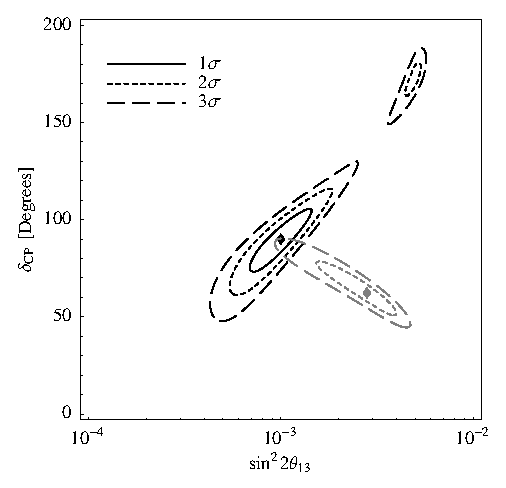
\includegraphics[width=7.5cm]{correntex}}
\end{center}

}

\index{norm}{Minimization!all-parameter}
The function to perform the all-parameter minimization is {\tt glbChiAll}:
\begin{function}
\GLBNS{ChiAll} 
{\tt double glbChiAll(const glb\_params in, glb\_params out, int exp)}
  returns the minimized $\chi^2$ over all parameters for the  experiment {\tt exp}. For the simulation of all initialized experiments,
use {\tt GLB\_ALL} for {\tt exp}. The values in {\tt in} are the guessed fit values for the minimizer. The actually determined parameters at the minimum are returned in {\tt out}. If {\tt out} is set to {\tt NULL}, this information will not be returned.
\end{function}
%
This function takes the suspected position of the local minimum and returns its actual position in {\tt out}, as well as the $\chi^2$-value 
at the minimum as return value. Thus, the return value can be immediately
used to judge whether the located degeneracy appears at the chosen
confidence level.

The example on page~\pageref{ex:sgndeg} illustrates how to locate the $\mathrm{sgn}(\ldm)$-degeneracy and show the corresponding degenerate solution in the $\stheta$-$\deltacp$-plane together with the original solution.
In this case, the position of the degeneracy can be easily guessed to be 
at the true parameter values but with inverted  $\ldm$.
The minimizer then runs off the plane of these parameters into the local minimum. It is very important to take into account the position of the degeneracy off this plane, since the actual $\chi^2$ in the minimum is probably lower than in the plane. Thus, the degeneracy may not even appear at the chosen confidence level in the plane, but it does appear at the real minimum. The two sections through the fit manifold shown in the figure on page~\pageref{ex:sgndeg} therefore do not appear at the same oscillation parameter values.\footnote{The discussed figure on page~\pageref{ex:sgndeg} is produced by  {\tt glbChiSys} and thus only represents a section through the fit manifold. For the projection including correlations, one may rather want to use {\tt glbChiTheta13Delta}.} 

\label{mass_ordering}
\index{norm}{Mass hierarchy}
\paragraph{Note:} Inverting the mass hierarchy is not
precisely the same as changing from $\Delta m^2_{31}
\rightarrow -\Delta m^2_{31}$.
In this case the absolute value of $\Delta m^2_{32}$ changes also, which
introduces a new frequency to the problem. Therefore, if we assume
normal hierarchy  whenever $\Delta m^2_{31}>0$, the corresponding
point in parameters space for inverted hierarchy is given by $\Delta 
m^2_{31}\rightarrow - \Delta m^2_{31} + \Delta m^2_{21}$, because
with this definition the absolute value of  $\Delta m^2_{32}$ is unchanged
and no new frequency is introduced.\\

\section{Advanced tricks for degeneracy localization$^*$}
\index{norm}{Advanced tricks}
For the more advanced reader, a number of tricks can be useful for the numerical localization of degenerate solutions. Here we give a qualitative, incomplete list:
\begin{description}
\item[Minimum $\boldsymbol{\chi^2}$ larger than threshold.] If a located degeneracy has a minimum $\chi^2$ larger than the corresponding confidence level threshold for the discussed quantity of interest, the degeneracy can be immediately ignored. This saves a lot of computation time.
\item[Locating degeneracies in more complicated topologies.] For more complicated topologies, such as for neutrino factories, it is often useful to use multi-step location procedures or analytical knowledge. For example, for a numerical procedure, one may first of all switch off the systematics and keep $\stheta$ or $\deltacp$ fixed, \ie, use {\tt glbChiTheta13}, where $\stheta$ or $\deltacp$ is fixed at the best-fit value. The result can then be used as a starting point for {\tt glbChiAll} for the individual experiments with the systematics switched on again. 
\item[Forcing the minimizer into the targeted solution.]
In addition to switching off the systematics, it can be useful to reduce the input errors during some steps of the localization process in order to prevent the minimizer from running away too far from the targeted solution.
The example on page~\pageref{ex:sgndeg} illustrates this with the
input error for $\ldm$: Since the guessed starting point might be
quite far away from the real degeneracy, the algorithm may in some cases
find the original solution instead of the degeneracy (which can
be immediately seen from the output vector). The input error
for $\ldm$ gives the algorithm a ``bias'' against the original solution.
However, note that the input error must not be too small in order
to avoid a significant contribution of the prior to the final $\chi^2$.
Alternatively, one could once again run {\tt glbChiAll} with the located 
minimum as {\tt in} vector, and $\ldm$ kept free.
\item[Finding degeneracies with multiple experiments.] For multiple experiments, it turns out to be useful to locate the degeneracies for individual experiments first. Then, all of the found degeneracies below the threshold can be tested for the combination of all experiments.
\item[Tracking algorithm.] If one scans a large portion of the parameter space with different input values, it is often useful to use the output from the previous minimization as educated guess for the next minimization. This works often very well if the degeneracy can be located in a part of the parameter space and the input parameter values change slowly enough (adiabatic transformation of the fit manifold). 
\item[Pre-scanning the parameter space.] In some cases, a very fast procedure can be a pre-scan 
of the relevant parameters using the very fast {\tt glbChiSys}. For example, for the intrinsic degeneracy, the location of the degeneracy in the $(\deltacp,\theta_{13})$ plane can easily and quickly found with {\tt glbChiSys} while keeping the other parameters fixed. Use this location then as a starting point for {\tt glbChiAll}.
\item[Manual scan of a subspace.] In some cases, the minimizer easily ends up in the wrong/unwanted solution, which is in most cases the already known best-fit solution. For example, when locating the octant degeneracy, it is difficult to prevent the minimizer from running into the best-fit octant. In this case, one can scan one parameter (such as $\theta_{23}$) on a grid by choosing only valid values, and use {\tt glbChiNP} to marginalize over the other ones (while keeping \eg\ $\theta_{23}$ fixed). Therefore, the 6-parameter minimization is split into a 1-parameter grid-based minimization and a 5-parameter simultaneous minimization. Advantage: Runs with all \GLOBES\ versions. Disadvantage: Very slow. 
\item[Using Schwetz-priors (\GLOBES\ 3.0 and higher).] An elegant and fast method to prevent the minimizer from running into parts of the parameter space is to use user-defined priors and add a penalty as soon as a taboo zone is entered (\cf, \Sec~\ref{sec:userdefined}). This method was initially suggested by Thomas Schwetz.
\item[Using total rates.] In order to systematically locate all degeneracies (the eight-fold degeneracy), relatively reliable methods use the total appearance neutrino and antineutrino event rates of the experiment to determine educated guesses. The method goes as follows: Plot the curves with equal total rate in the $\sin^2 2 \theta_{13}$-$\delta_{\mathrm{CP}}$-plane for both neutrinos and antineutrinos using the same rates as in the best-fit point. The curves will intersect at the intrinsic degeneracy (if it all). Plot the same curves for the same rates with $\mathrm{sgn}(\Delta m_{31}^2)$ flipped. Again you will find a maximum of two intersection points. Now do the same for $\pi/2 - \theta_{23}$ flipped, and for  $\mathrm{sgn}(\Delta m_{31}^2)$ combined with $\pi/2 - \theta_{23}$ flipped (mixed degeneracy). You will find at most two more intersection points in each case.
The results should look somewhat like this, where the best-fit point is not marked\footnote{The marks correspond to the points where the discrete degeneracies are located according to this specific algorithm. Note that
one also wants to find the positions of close-to-intersections, because statistical errors may be as large
as that the corresponding degenerate solution may still be present at the chosen confidence level.
Therefore, in the third plot these close-to-intersections are marked as well.}:
\begin{center}
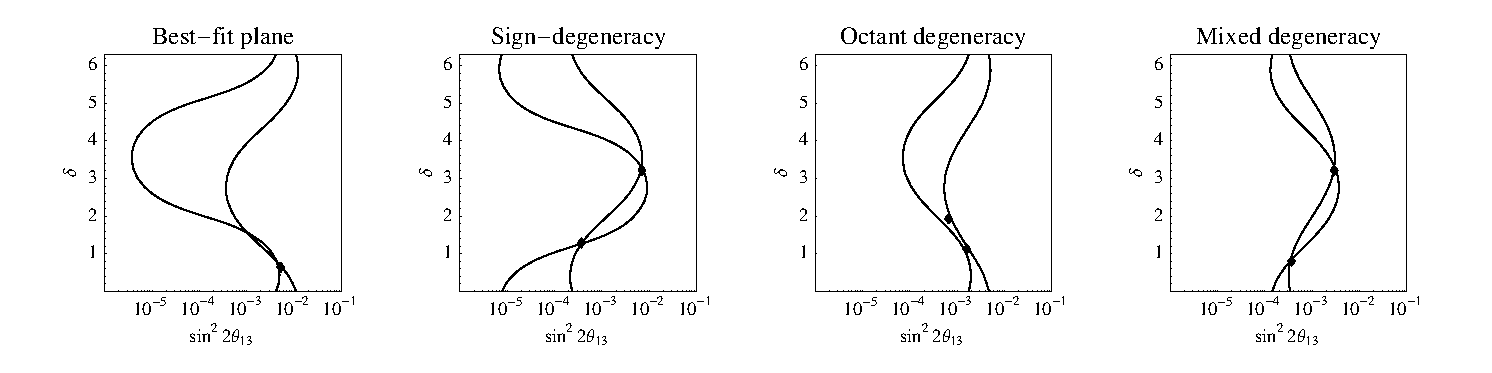
\includegraphics[width=0.95\textwidth]{ircurves}
\end{center}
 Altogether, there is a maximum of eight intersection points in the $\sin^2 2 \theta_{13}$-$\delta_{\mathrm{CP}}$-plane, one of which is the best-fit point. These points can be used as starting points for the minimizer to locate the eight-fold degeneracy. Note that similar methods using the $\chi^2$ instead of the total rates have also been successfully used in the past.  In this case, one would scan for local minimas
disconnected from the best-fit solution.
\end{description}
Finally, note that any degenerate solution below the confidence level threshold, which cannot be located, makes the result appear better than it actually is. Thus, one should be careful with the determination of the degenerate solutions in order to find all of them.
\index{norm}{Degeneracies|)}


%%%%%%%%%%%%%%%%%%%%%%%%%%%%%%%%%%%%%%%%%%%%%%%%%%%%%%%%%%%%%%%%%%%%%%%%%%
\chapter{Obtaining low-level information}
\index{norm}{Low-level information}

In this chapter, we discuss possibilities to obtain low-level information
in \GLOBES , \ie, oscillation probabilities, rates, and other
information lower than on the $\chi^2$-level.

\section{Oscillation probabilities}
\index{norm}{Oscillation!probabilities}

\GLOBES\ can compute the probabilities in vacuum
with the following function:
\begin{function}
\GLBNS{VacuumProbability}
{\tt double glbVacuumProbability(int l, int m, int panti,double E, double L)} returns the neutrino oscillation probability $\nu_l \rightarrow \nu_m$ for the energy {\tt E} and the baseline {\tt L} in vacuum. The parameter
{\tt panti} is $+1$ for neutrinos and $-1$ for antineutrinos. 
\end{function}
Note that for this and the other probability functions $1 \le$ {\tt l}, {\tt m} $\le 3$.
In addition, the oscillation probabilities in matter can be obtained
with:
\begin{function}
\GLBNS{ProfileProbability}
{\tt double glbProfileProbability(int exp, int l, int m, int panti,double E)} returns the neutrino oscillation probability $\nu_l \rightarrow \nu_m$ for the energy {\tt E} in matter, where the matter density profile
is the one of experiment {\tt exp}. The parameter
{\tt panti} is $+1$ for neutrinos and $-1$ for antineutrinos.
\end{function}
This function ignores the filter state, and it does not use the filter if switched on.
For a constant matter density profile, it is sufficient to specify the oscillation channel with
\begin{function}
\GLBNS{ConstantDensityProbability}
{\tt double glbConstantDensityProbability(int l, int m, int panti, double E, double L, double rho)} returns the neutrino oscillation probability $\nu_l \rightarrow \nu_m$ for the energy {\tt E} in constant matter, where the matter density profile
has the constant density {\tt rho} and the baseline is {\tt L}. The parameter
{\tt panti} is $+1$ for neutrinos and $-1$ for antineutrinos.
\end{function}
If one in addition wants to use the low-pass filter feature in \GLOBES\ (see \Sec~\ref{sec:energy}), one can can use
\begin{function}
\GLBNS{FilteredConstantDensityProbability}
{\tt double glbFilteredConstantDensityProbability(int exp, int l, int m, int panti, double E)} returns the neutrino oscillation probability $\nu_l \rightarrow \nu_m$ for the energy {\tt E} in constant matter, where the matter density and baseline, as well as the filter properties are taken from experiment {\tt exp}. The parameter {\tt panti} is $+1$ for neutrinos and $-1$ for antineutrinos.
\end{function}
This function uses the filter depending on the filter state, \ie, if it is switched off, it will not be used.

%%%%%%%%%%%%%%%%%%%%%%%%%%%%%%%%%%%%%%%%%%%%%%%%%%%%%%%%%%%%
\section{Information from \AEDL\ files$^*$}
\label{sec:aedl_names}

In some cases, it is necessary to obtain information from the loaded \AEDL\
files. This and the next sections are marked as advanced because knowledge of \AEDL\ is
required, \ie,  the reader should be familiar with Part~\ref{part:2} of the manual.
%
Very basic information is supplied with
\begin{function}
\GLBNS{GetEminEmax}
{\tt int glbGetEminEmax(int experiment, double *emin, double *emax)} returns the
energy range [{\tt emin}, {\tt emax}] covered by the binning as defined in the \AEDL\ file for the experiment
{\tt experiment}.
\end{function}
\begin{function}
\GLBNS{GetEnergyWindow}
{\tt int glbGetEnergyWindow(int exp, int rule, double *low, double *high)} returns the
energy window [{\tt low}, {\tt high}] defined in the \AEDL\ file for the experiment
{\tt exp} and rule {\tt rule}.
\end{function}
\begin{function}
\GLBNS{GetEnergyWindowBins}
{\tt int glbGetEnergyWindowBins(int exp, int rule, int *lowbin, int *highbin)} returns the
energy window in terms of bin numbers [{\tt lowbin}, {\tt highbin}] corresponding to the energy window defined in the \AEDL\ file for the experiment {\tt exp} and rule {\tt rule}.
\end{function}
\begin{function}
\GLBNS{GetNumberOfBins}
{\tt int glbGetNumberOfBins(int exp)} returns the number of bins for the experiment {\tt exp}.
\end{function}
\begin{function}
\GLBNS{GetNumberOfSamplingPoints}
{\tt int glbGetNumberOfSamplingPoints(int exp)} returns the number of sampling points for the experiment {\tt exp}.
\end{function}
\begin{function}
\GLBNS{GetBinSizeListPtr}
{\tt double *glbGetBinSizeListPtr(int exp)} returns a pointer to the array of bin widths
for the experiment {\tt exp}.
\end{function}
\begin{function}
\GLBNS{GetSamplingStepsizeListPtr}
{\tt double *glbGetSamplingStepsizeListPtr(int exp)} returns a pointer to the array of
sampling step sizes for the experiment {\tt exp}.
\end{function}
\begin{function}
\GLBNS{GetBinCentersListPtr}
{\tt double *glbGetBinCentersListPtr(int exp)} returns a pointer to the array of
mean bin energies for the experiment {\tt exp}.
\end{function}
\begin{function}
\GLBNS{GetSamplingPointsListPtr}
{\tt double *glbGetSamplingPointsListPtr(int exp)} returns a pointer to the array of
sampling points for the experiment {\tt exp}.
\end{function}

In order to obtain information on the structure of the rules, 
a number of functions are provided:
\begin{function}
\GLBNS{GetNumberOfRules}
{\tt int glbGetNumberOfRules(int exp)} returns the number of
rules in experiment {\tt exp}.
\end{function}
\begin{function}
\GLBNS{GetLengthOfRule}
{\tt int glbGetLengthOfRule(int exp, int rule, int signal)} returns
the length of rule {\tt rule} in experiment {\tt exp}. The parameter
{\tt signal} can be either \GLBC{GLB\_SIG} for the number of signal
components or \GLBC{GLB\_BG} for the number of background components.
\end{function}
% NOT DOCUMENTED, BECAUSE THESE NORMALIZATIONS ARE NOW PRE-DEFINED:
%
% \begin{function}
% \GLBNS{GetNormalizationInRule}
% {\tt double glbGetNormalizationInRule(int exp, int rule, int signal)}
% returns the normalization (normalization or background center)
% in rule {\tt rule} of the experiment {\tt exp}.
% The parameter {\tt signal} refers to signal (\GLBC{GLB\_SIG}) or background
% (\GLBC{GLB\_BG}).
% \end{function}
\begin{function}
\GLBNS{GetChannelInRule}
{\tt int glbGetChannelInRule(int exp, int rule, int pos, int signal)}
returns the channel number in rule {\tt rule} at the position {\tt pos}
of the experiment {\tt exp}.
The parameter {\tt signal} refers to signal (\GLBC{GLB\_SIG}) or background
(\GLBC{GLB\_BG}).
\end{function}
\begin{function}
\GLBNS{GetCoefficientInRule}
{\tt double glbGetCoefficientInRule(int exp, int rule, int pos, int signal)}
returns the coefficient of the component {\tt pos} in rule {\tt rule} 
of the experiment {\tt exp}.
The parameter {\tt signal} refers to signal (\GLBC{GLB\_SIG}) or background
(\GLBC{GLB\_BG}).
\end{function}
%
Similarly to the rules, one can find the number of channels of an experiment:
\begin{function}
\GLBNS{GetNumberOfChannels}
{\tt int glbGetNumberOfChannels(int exp)} returns the number of 
channels of experiment {\tt exp}.
\end{function} 
For each channel, the efficiencies and backgrounds can be returned with the following functions:
\begin{function}
\GLBNS{GetEfficiencyPtr}
{\tt double *glbGetEfficiencyPtr(int exp, int ch, int pre\_post)} returns a pointer to
the efficiency list for experiment {\tt exp} and channel {\tt ch}. The pre- or post-smearing
efficiencies are returned with {\tt pre\_post} set to {\tt GLB\_PRE} and {\tt GLB\_POST}, respectively.
\end{function}
\begin{function}
\GLBNS{GetBackgroundPtr}
{\tt double *glbGetBackgroundPtr(int exp, int ch, int pre\_post)} returns a pointer to
the background list for experiment {\tt exp} and channel {\tt ch}. The pre- or post-smearing
backgrounds are returned with {\tt pre\_post} set to {\tt GLB\_PRE} and {\tt GLB\_POST}, respectively.
\end{function}

\index{norm}{AEDL@\AEDL!names}
Since in \AEDL\, rules, cross section, fluxes etc. carry a `name' by
which they can be referred to, while in C they carry only an integer
index, it is sometimes difficult to figure out the correct correspondence.
Therefore the information about this correspondence obtained during
parsing is stored and can be accessed within C by the following two functions.
\begin{function}
\GLBNS{NameToValue}
{\tt int glbNameToValue(int exp, const char* context, const char *name)}
Converts an \AEDL\ name given as argument {\tt name} into the corresponding
C index. The variable {\tt context} describes wether this name belongs
to a rule, channel, flux, energy, or cross type environment. {\tt exp}
is the number of the experiment and can not be {\tt GLB\_ALL}. It returns
either the index in case of success or {\tt -1} in case the name was not
found. 
\end{function}

\begin{function}
\GLBNS{ValueToName}
{\tt const char *glbValueToName(int exp,const char* context, int value)}
Converts a C index given as argument {\tt value} into the corresponding 
\AEDL\ name. The variable {\tt context} describes wether the index belongs
to a rule, channel, flux, energy or cross type environment. {\tt exp}
is the number of the experiment and can not be {\tt GLB\_ALL}. It returns
either the name in case of success or {\tt NULL} in case the name was not
found. The returned string must not be modified.
\end{function}




%%%%%%%%%%%%%%%%%%%%%%%%%%%%%%%%%%%%%%%%%%%%%%%%%%%%%%%%%%%%%
\section{Event rates$^*$}
\index{norm}{Event rates}
\label{sec:event_rates}
One can also return event rates in \GLOBES , but this feature
requires some knowledge about the experiment definition. 
In fact, many of these functions are very advanced, which means
that the reader who wants to use them should be familiar with
\Secs~\ref{sec:channel} and~\Sec~\ref{sec:rules} of the \AEDL\ manual.
Note that parts of the event rate access have changed in \GLOBES\ 3.0,
because user-defined systematics require very fast access, which was
not possible with the old method.

A very simple function is for the total rate
\begin{function}
\GLBNS{TotalRuleRate}
{\tt double glbTotalRuleRate(int exp, int rule, int pos,
int effi, int bgi, int coeffi, int signal)} returns the total rates.
A specific experiment {\tt exp} and a 
specific rule {\tt rule} have to be chosen, as well as the signal
or background rate {\tt signal} (either \GLBC{GLB\_SIG} or \GLBC{GLB\_BG}).
The position {\tt pos} refers to the component within the signal or 
background, and can also be {\tt GLB\_ALL}. The function may return
the rates with (\GLBC{GLB\_W\_COEFF}) or without (\GLBC{GLB\_WO\_COEFF})
overall efficiency coefficient, as it is specified by {\tt coeffi}. 
In addition, it may contain the post-smearing efficiencies (set
{\tt effi} to \GLBC{GLB\_W\_EFF} or \GLBC{GLB\_WO\_EFF}), and the
post-smearing backgrounds (set
{\tt bgi} to \GLBC{GLB\_W\_BG} or \GLBC{GLB\_WO\_BG}). The pre-smearing
efficiencies and backgrounds cannot be accessed at the rule level.
\end{function}
The function {\tt glbTotalRuleRate} is especially useful if
one wants to draw bi-rate graphs with total event rates, or look
for the $(\deltacp,\theta_{13})$-degeneracy by the intersection of 
neutrino and antineutrino constant event rate curves.

There are several functions to directly print or save the event rate
information:
\begin{function}
\GLBNS{ShowRuleRates}
{\tt int glbShowRuleRates(FILE* stream, int exp, int rule, int pos,
int effi, int bgi, int coeffi, int signal)} prints the binned rule rates as
a list with energy and event rate to the file {\tt stream} (either an
open file, or {\tt stdout}). A specific experiment {\tt exp} and a 
specific rule {\tt rule} have to be chosen, as well as the signal
or background rate {\tt signal} (either \GLBC{GLB\_SIG} or \GLBC{GLB\_BG}).
The position {\tt pos} refers to the component within the signal or 
background, and can also be {\tt GLB\_ALL}. The function may return
the rates with (\GLBC{GLB\_W\_COEFF}) or without (\GLBC{GLB\_WO\_COEFF})
overall efficiency coefficient, as it is specified by {\tt coeffi}. 
In addition, it may contain the post-smearing efficiencies (set
{\tt effi} to \GLBC{GLB\_W\_EFF} or \GLBC{GLB\_WO\_EFF}), and the
post-smearing backgrounds (set
{\tt bgi} to \GLBC{GLB\_W\_BG} or \GLBC{GLB\_WO\_BG}). The pre-smearing
efficiencies and backgrounds cannot be accessed at the rule level.
The return value
is $0$ if successful, and $-1$ if unsuccessful.
\end{function}
\begin{function}
\GLBNS{ShowChannelRates}
{\tt int glbShowChannelRates(FILE *stream,
int exp, int channel, int smearing, int effi, int bgi)}
prints the binned channel rates as
a list with energy and event rate to the file {\tt stream} (either an
open file, or {\tt stdout}). A specific experiment {\tt exp} and a 
specific channel {\tt channel} have to be chosen.
The function may return
the rates before (\GLBC{GLB\_PRE}) or after (\GLBC{GLB\_POST})
the energy smearing, as it is specified by {\tt smearing}.
In addition, it may contain the pre- and post-smearing efficiencies (set
{\tt effi} to \GLBC{GLB\_W\_EFF} or \GLBC{GLB\_WO\_EFF}), and the
pre- and post-smearing backgrounds (set
{\tt bgi} to \GLBC{GLB\_W\_BG} or \GLBC{GLB\_WO\_BG}). Note that
the post-smearing efficiencies and backgrounds cannot be taken into
account if the rates are returned before the energy smearing.
The return value
is $0$ if successful, and $-1$ if unsuccessful.
\end{function}

\index{norm}{Event rates}
For rate vectors, \GLOBES\ currently supports rule-based and channel-based event rate functions, where typically pointers on the rate vectors are returned. The following pointer-based functions are currently supported:
\begin{function}
\GLBNS{GetChannelRatePtr}
{\tt double *glbGetChannelRatePtr(int exp, int ch, int pre\_post)} returns a 
pointer to the simulated rate vector of experiment {\tt exp} and channel {\tt ch}. Either
pre-smearing ({\tt pre\_post} is {\tt GLB\_PRE}) or post-smearing ({\tt pre\_post} is {\tt GLB\_POST})
rates can be accessed.
\end{function}
\begin{function}
\GLBNS{GetRuleRatePtr}
{\tt double *glbGetRuleRatePtr(int exp, int rule)} returns a 
pointer to the simulated rate vector of experiment {\tt exp} and rule {\tt rule}.
\end{function}
\begin{function}
\GLBNS{GetSignalRatePtr}
{\tt double *glbGetSignalRatePtr(int exp, int rule)} returns a 
pointer to the simulated signal rate vector of experiment {\tt exp} and rule {\tt rule}.
\end{function}
\begin{function}
\GLBNS{GetBGRatePtr}
{\tt double *glbGetBGRatePtr(int exp, int rule)} returns a 
pointer to the simulated background rate vector of experiment {\tt exp} and rule {\tt rule}.
\end{function}
\begin{function}
\GLBNS{GetChannelFitRatePtr}
{\tt double *glbGetChannelFitRatePtr(int exp, int ch, int pre\_post)} returns a 
pointer to the fit rate vector of experiment {\tt exp} and channel {\tt ch}. Either
pre-smearing ({\tt pre\_post} is {\tt GLB\_PRE}) or post-smearing ({\tt pre\_post} is {\tt GLB\_POST})
rates can be accessed.
\end{function}
\begin{function}
\GLBNS{GetSignalFitRatePtr}
{\tt double *glbGetSignalFitRatePtr(int exp, int rule)} returns a 
pointer to the fit signal rate vector of experiment {\tt exp} and rule {\tt rule}.
\end{function}
\begin{function}
\GLBNS{GetBGFitRatePtr}
{\tt double *glbGetBGFitRatePtr(int exp, int rule)} returns a 
pointer to the fit background rate vector of experiment {\tt exp} and rule {\tt rule}.
\end{function}
A simple example how to use these functions to print a rate vector is
\begin{quote}
{\tt
 int i; \\
   int n\_bins = glbGetNumberOfBins(EXP\_FAR); \\
  double *true\_rates\_N = glbGetRuleRatePtr(0, 0); \\
  printf("Simulated rates, experiment 0, rule 0: $\backslash$n"); \\
  for(i=0;i<n\_bins;i++) printf("\% g ",true\_rates\_N[i]); \\
  printf("$\backslash$n");
}
\end{quote}

% OLD FUNCTIONS:
% \begin{function}
% \GLBNS{GetChannelRates}
% {\tt int glbGetChannelRates(double** data,
% size\_t* length, int exp, int channel, int smearing)}
% writes the binned raw channel rates to the list {\tt data}
% and the length of this list to {\tt length}. 
% A specific experiment {\tt exp} and a 
% specific channel {\tt channel} have to be chosen.
% The function may return
% the rates before ({\tt smearing} is \GLBC{GLB\_PRE}) or after ({\tt smearing} is \GLBC{GLB\_POST})
% the energy smearing, where no user-defined data
% (pre-/post-smearing efficiencies or backgrounds) are taken into account.
% The return value is $-1$ if unsuccessful.
% \end{function}
% \begin{function}
% \GLBNS{GetUserData}
% {\tt int glbGetUserData(double** data,
% size\_t* length, int exp, int channel, int smearing, int bgeff)}
% writes the binned user-defined backgrounds or efficiencies 
% to the list {\tt data} and the length of this list to {\tt length}. 
% A specific experiment {\tt exp} and a 
% specific channel {\tt channel} have to be chosen.
% The function may return
% the pre- ({\tt smearing} is \GLBC{GLB\_PRE}) or post- ({\tt smearing} is \GLBC{GLB\_POST}) smearing backgrounds ({\tt bgeff} is \GLBC{GLB\_BG}) 
% or efficiencies ({\tt bgeff} is \GLBC{GLB\_EFF}). 
% The return value is $-1$ if unsuccessful.
% \end{function}
% Since \GLOBES\ reserves the memory for the lists returned in these
% functions, which it allocates on an internal stack, one has to reset
% the stack at the end of the rates access with
% \begin{function}
% \GLBNS{ResetRateStack}
% {\tt void glbResetRateStack()} resets the rate stack used for the
% lists returned from {\tt glbGetChannelRates} or {\tt glbGetUserData}.
% \end{function}
% A code excerpt to show the channel rates may look like this:
% \begin{quote}
% {\tt
%  double* rates; \\
%   size\_t length; \\
%   glbGetChannelRates(\&rates,\&length,0,0,GLB\_PRE); \\
%   int i; \\
%   for(i=0;i<length;i++) printf("\%g $\backslash$n",rates[i]); \\
%   glbResetRateStack(); \\
% }
% \end{quote}

\section{Fluxes and cross sections$^*$}
\index{norm}{Flux} \index{norm}{Cross section}

Another piece of low-level information, which can be returned by \GLOBES ,
are the numbers from the loaded fluxes and cross sections.
The following functions interpolate on the loaded fluxes and cross 
sections, \ie, any value in the allowed energy range can be given as input:
\begin{function}
\GLBNS{Flux}
{\tt double glbFlux(int exp, int ident, 
double E, double distance, int l, int anti)} returns
the flux of flux number {\tt ident} of the experiment {\tt exp}
for the flavor $\nu_l$ 
and polarity {\tt anti} ($+1$: neutrinos, $-1$: antineutrinos) at the energy {\tt E} and distance {\tt distance}.
\end{function}

\begin{function}
\GLBNS{XSection}
{\tt double glbXSection(int exp, 
int ident, double E, int l, int anti)} returns
the cross section of experiment {\tt exp}, 
cross section number {\tt ident} for the flavor $\nu_l$ and polarity {\tt anti} ($+1$: neutrinos, $-1$: antineutinos) at the energy {\tt E}.
\end{function}
%
The number of fluxes can be obtained with
\begin{function}
\GLBNS{GetNumberOfFluxes}
{\tt int glbGetNumberOfFluxes(int exp)} returns the number of 
fluxes defined in experiment {\tt exp}.
\end{function}



%%%%%%%%%%%%%%%%%%%%%%%%%%%%%%%%%%%%%%%%%%%%%%%%%%%%%%%%%%%%%%%%%%%%%%%%%
\chapter{Changing experiment parameters at running time}
\label{chapt:running}
\index{norm}{Experiment parameters}

Many of the parameters in experiment definitions can be changed
at running time. For example, we have introduced in 
\Sec~\ref{sec:luminosity} possibilities to change the integrated
luminosity, which consists of source power, running time, and target mass.
In this chapter, we discuss more sophisticated
experiment changes. However, since \GLOBES\ computes a lot of
information only once when an experiment is loaded, many
parameters can not be changed at running time. For example,
the energy resolution function or the number of bins are used
to compute the smearing matrix already at the initialization
of the experiment, which saves a lot of computation
time for most applications. In \Sec~\ref{sec:aedlparams}, we 
introduce a mechanism how one can even change these \AEDL\ parameters
during running time.


\section{Systematics}
\label{sec:systematics}
\index{norm}{Systematics}
\index{norm}{Systematics!on/off}

Changing the systematics at running time can be useful to investigate
the impact factors affecting the measurement.
In \GLOBES , the systematics is defined rule-based, \ie, each rule
has its own systematics. 
In addition, \GLOBES\ supports dual systematics, \ie, \AEDL\ requires that it has to be
defined in each rule what ``Systematics on'' and ``Systematics off'' means.
In principle, these two sets correspond to two completely different systematics
implementations, and it is up to the \AEDL\ authors to define what that means.
From the point of view of the API, it is very simple to switch the systematics on and off, \ie,
to switch between the two systematics modes:
\begin{function}
\GLBNS{SwitchSystematics}
{\tt int glbSwitchSystematics(int exp, int rule, int on\_off)}
switches the systematics in experiment {\tt exp} and rule {\tt rule}
on ({\tt on\_off} is \GLBC{GLB\_ON}) or off ({\tt on\_off} is \GLBC{GLB\_OFF}). For the experiment or
rule index, one can also use \GLBC{GLB\_ALL}. 
\end{function}
One can also return the systematics state with
\begin{function}
\GLBNS{GetSysOnOffState}
{\tt int glbGetSysOnOffState(int exp, int rule)}
returns the systematics state in experiment {\tt exp} and rule {\tt rule}. 
\end{function}
In the example on page~\pageref{ex:barcharts}, the application of
{\tt glbSwitchSystematics} is demonstrated to show the impact of
systematics, correlations, and degeneracies.

\example{The impact of systematics, correlations, and degeneracies}{
\label{ex:barcharts}
\index{norm}{Bar plots}
\index{norm}{Systematics!on/off}
Here, we demonstrate how systematics, correlations, and degeneracies
can be successively included in the calculation of the $\stheta$-sensitivity limit.
The following code fragment shows how systematics can be switched off
in order to compute the sensitivity limit from statistics only:
\begin{quote}
{\tt 
/* Calculate chi2 with statistics only */ \\
double CalcNoSystematics(double theldm,double thex) \\
\{ \\
\hspace*{0.5cm} /* Switch systematics off for all exps and all rules */ \\
\hspace*{0.5cm} glbSwitchSystematics(GLB\_ALL,GLB\_ALL,GLB\_OFF); \\
\\
\hspace*{0.5cm} /* Calculate Chi2-list as if systematics were on */ \\
\hspace*{0.5cm} double res=CalcSystematics(theldm,thex); \\
\\
\hspace*{0.5cm} /* Switch systematics on for all exps and all rules */ \\
\hspace*{0.5cm} glbSwitchSystematics(GLB\_ALL,GLB\_ALL,GLB\_ON); \\
\\
\hspace*{0.5cm} return res; \\
\} \\
}
\end{quote}

\vspace*{-0.5cm}

The complete code is very advanced and can be found in {\tt example4.c}.
It includes many concepts from earlier examples, and, in addition,
it uses a little trick: It avoids falling into the wrong solution with
{\tt glbChiTheta13} by using the fit value of $\deltacp$ from the step
before as prediction for the position of the minimum in the current calculation.

The returned lists of data from the example represent $\chi^2$ 
as function of the fit value of $\stheta$. The intersections of these
curves with the line $\chi^2 = 9$ give the $\stheta$ sensitivity
limits at the $3 \sigma$ confidence level. Note that, in the following
plot, the $\mathrm{sgn}(\ldm)$- and $(\deltacp,\theta_{13})$-degeneracies
are not included in the sensitivity limit with correlations only (green bar),
but only in the limit with degeneracies (yellow bar):
\begin{center}
\colorbox{white}{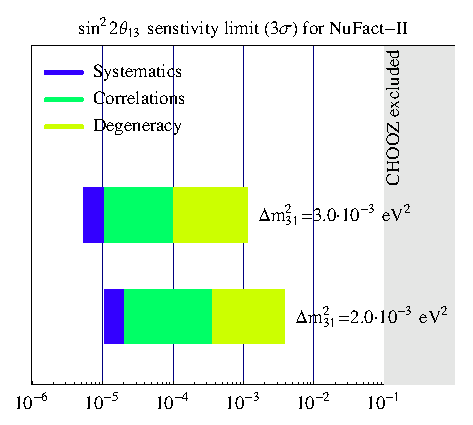
\includegraphics[width=6.5cm]{barsex}}
\end{center}
}

The following material requires knowledge of \AEDL , which means that it can be skipped
at a first reading. 
%
During running time, it is possible to change the systematics of an experiment or
rule (as compared to the systematics assigned in the \AEDL\ file) with the following function:
\begin{function}
\GLBNS{SetChiFunction}
{\tt int glbSetChiFunction(int exp, int rule, int on\_off, const char *name, double *errors)}
 tells \GLOBES\ to use the registered user-defined systematics identified by the string {\tt name}
or any built-in systematics
to calculate $\chi^2$ for the experiment {\tt exp} and the rule {\tt rule}. 
Both of the parameters {\tt exp} and {\tt rule} can take the value \GLBC{GLB\_ALL} to specify that the
given systematics function should be used for each experiment or each rule. The parameter 
{\tt on\_off} determines if the systematics function should be used when systematical errors
are switched on ({\tt GLB\_ON}), or when they are switched off ({\tt GLB\_OFF}).
The array {\tt errors} sets the systematical errors in the order in which they
are expected by the systematics function (indices run from $0$ to
the number of systematics parameters-1). The function returns zero, if successful.
\end{function}
Note that user-defined systematics functions have to be registered with \GLB{DefineChiFunction} first. 
One can also request the systematics function by 
\begin{function}
\GLBNS{GetChiFunction}
{\tt int glbGetChiFunction(int exp, int rule, int on\_off, char *sys\_id, size\_t max\_len)}
returns the name of the systematics $\chi^2$ function of a given experiment {\tt exp} and rule {\tt rule} for
systematics on or off as given by {\tt on\_off}. The name is copied to the string
{\tt sys\_id}, the maximum length of which is specified by {\tt max\_len}. If
{\tt max\_len} is too small, or if any other error occurs, the return value is $< 0$.
\end{function}

% \index{norm}{Error dimension}
% The error dimension (for the definition, see \Sec~\ref{sec:rules}) can also be accessed directly with 
% \begin{function}
% \GLBNS{SetErrorDim}
% {\tt int glbSetErrorDim(int exp, int rule, int on\_off, int value)}
% sets the error dimension for systematics on ({\tt on\_off} is \GLBC{GLB\_ON}) or off ({\tt on\_off} is \GLBC{GLB\_OFF}) of experiment {\tt exp} and rule {\tt rule} to the value {\tt value}. The function returns
% $-1$ if not successful.
% \end{function}
% \begin{function}
% \GLBNS{GetErrorDim}
% {\tt int glbGetErrorDim(int exp, int rule, int on\_off)}
% returns the error dimension for systematics on ({\tt on\_off} is \GLBC{GLB\_ON}) or off ({\tt on\_off} is \GLBC{GLB\_OFF}) of experiment {\tt exp} and rule {\tt rule}.
% \end{function}

\index{norm}{Signal!errors}
\index{norm}{Background!errors}
\index{norm}{Background!centers}
Except from the general treatment of systematics, one can read out
and change the signal and background errors for standard pre-defined systematics
during running time:
\begin{function}
\GLBNS{SetSignalErrors}
{\tt int glbSetSignalErrors(int exp, int rule, double norm, double tilt)}
sets the signal errors of experiment {\tt exp} and rule {\tt rule}
to {\tt norm} (normalization error) and {\tt tilt} (tilt/calibration error).
\end{function}
\begin{function}
\GLBNS{GetSignalErrors}
{\tt int glbGetSignalErrors(int exp, int rule, double* norm, double* tilt)}
writes the signal errors of experiment {\tt exp} and rule {\tt rule}
to {\tt norm} (normalization error) and {\tt tilt} (tilt/calibration error).
\end{function}
\begin{function}
\GLBNS{SetBGErrors}
{\tt int glbSetBGErrors(int exp, int rule, double norm, double tilt)}
sets the background errors of experiment {\tt exp} and rule {\tt rule}
to {\tt norm} (normalization error) and {\tt tilt} (tilt/calibration error).
\end{function}
\begin{function}
\GLBNS{GetBGErrors}
{\tt int glbGetBGErrors(int exp, int rule, double* norm, double* tilt)}
writes the background errors of experiment {\tt exp} and rule {\tt rule}
to {\tt norm} (normalization error) and {\tt tilt} (tilt/calibration error).
\end{function}
% ELIMINATED FROM DOC, BECAUSE WE WANT TO AVOID THE BG CENTERS IN THE FUTURE (CONFUSION) [WW]
%
% \begin{function}
% \GLBNS{SetBGCenters}
% {\tt int glbSetBGCenters(int exp, int rule, double norm, double tilt)}
% sets the background centers of experiment {\tt exp} and rule {\tt rule}
% to {\tt norm} (normalization center) and {\tt tilt} (tilt/calibration center).
% \end{function}
% \begin{function}
% \GLBNS{GetBGCenters}
% {\tt int glbGetBGCenters(int exp, int rule, double* norm, double* tilt)}
% writes the background centers of experiment {\tt exp} and rule {\tt rule}
% to {\tt norm} (normalization center) and {\tt tilt} (tilt/calibration center).
% \end{function}
As a more flexible concept, the systematical errors may be given as lists for
both user-defined and built-in systematics. For example, the standard signal and background
pre-defined errors can be accessed as lists with four elements (signal
normalization, signal tilt, background normalization, background tilt) if built-in
systematics is used. The corresponding 
functions are:
\begin{function}
\GLBNS{SetSysErrorsList} 
{\tt int glbSetSysErrorsList(int exp, int rule, int on\_off, const double *sys\_list)}
changes the systematical errors defined in the \AEDL\ file in experiment {\tt exp} and 
rule {\tt rule} to the values in {\tt sys\_list}. This change can be perfomed for
systematics on or systematics off by using {\tt GLB\_ON} or {\tt GLB\_OFF} for {\tt on\_off}. 
\end{function}
\begin{function}
\GLBNS{GetSysErrorsListPtr} 
{\tt double* glbGetSysErrorsListPtr(int exp, int rule, int on\_off)}
returns a pointer to the list of systematical errors as defined in the \AEDL\ file in experiment {\tt exp} and 
rule {\tt rule}. Choose
systematics on or systematics off by using {\tt GLB\_ON} or {\tt GLB\_OFF} for {\tt on\_off}. 
\end{function}
As usual, all these functions return $-1$ if they were not successful.
%.
For user-defined systematics, see \Sec~\ref{sec:userchi}, and 
for the definitions of these quantities, see \Sec~\ref{sec:rules}. 

\section{Baseline and matter density profile$^*$}
\label{sec:baselinemd}
\index{norm}{Baseline!change}
\index{norm}{Matter density!change profile}

In order to change the baseline of an experiment, it is important
to keep in mind that each experiment has a profile type defined
in the \AEDL\ file (average density, PREM profile with a given
number of steps, or arbitrary profile; \cf, \Tab~\ref{tab:profiletypes}). One can check the currently
used profile type with
\begin{function}
\GLBNS{GetProfileTypeInExperiment}
{\tt int glbGetProfileTypeInExperiment(int exp)} returns the matter density profile
type of experiment {\tt exp}.
\end{function}
For each profile type, one can easily change the baseline with {\tt glbSetBaselineInExperiment},
where the average density or the PREM profile are re-computed, or the
steps in the arbitrary profile are re-scaled. If this behavior is 
not the desired one, one has to use {\tt glbSetProfilDataInExperiment}
as explained below.
\begin{function}
\GLBNS{SetBaselineInExperiment}
{\tt int glbSetBaselineInExperiment(int exp, double baseline)}
sets the baseline length in experiment {\tt exp} to {\tt baseline}.
The function returns $-1$ if it was not successful.
\end{function}
Note that {\tt glbSetBaselineInExperiment} does not change the
profile type in the experiment. The counterpart of this function is:
\begin{function}
\GLBNS{GetBaselineInExperiment} 
{\tt double glbGetBaselineInExperiment(int exp)} returns the
baseline length currently used for experiment {\tt exp}.
\end{function}
One can not change the profile type of an experiment manually
during running time. However, one can change the matter density
profile, where the profile type is automatically switched to 3, \ie\ 
arbitrary matter density profile. In addition, a number of functions 
are provided to compute possible matter density profiles (average density,
PREM profile). In general, a matter density profile in \GLOBES\ with
$N$ layers is represented by a list of lengths 
\begin{equation}
\mathrm{Lengths} = (x_1,x_2, \hdots, x_N) 
\end{equation}
and a list of densities
\begin{equation}
\mathrm{Densities} = (\rho_1,\rho_2, \hdots, \rho_N), 
\end{equation}
where the baseline is given by
\begin{equation}
L = \sum\limits_{i=1}^N x_i.
\end{equation}
In C, lists are represented as pointers to the first element:
\begin{quote}
{\tt  
  double* lengths; \\
  double* densities;
}
\end{quote}
Many of the \GLOBES\ baseline functions take and return
such lists as parameters, and are therefore more sophisticated
to handle. In general, any function
{\em returning} lists allocates the memory for them.
It is then up to the user to free this memory!
In addition, they normally provide the length of the lists $N$
by means of an additional argument which is a pointer to {\tt size\_t}. 
Normally, it is enough to declare
a variable of the type {\tt size\_t} and to give its address to the function.
The following functions return matter density profiles:
\begin{function}
\GLBNS{LoadProfileData}
{\tt int glbLoadProfileData(const char* filename, size\_t *layers, double **lengths, double **densities)} loads a density file from the file
{\tt filename}. It returns the number of layers {\tt layers}, the
list of lengths {\tt lengths}, and the list of densities {\tt densities}.
\end{function}
The file should contain in each line a length and density for one layer,
which are separated by an empty space.
\begin{function}
\GLBNS{StaceyProfile}
{\tt int glbStaceyProfile(double baseline, size\_t layers, double **lengths, double **densities)} creates a PREM/Stacey matter density profile with a
number of {\tt layers} steps for the baseline {\tt baseline}. The list of lengths {\tt lengths} and the list of densities {\tt densities} are returned.
\end{function}
Note that this function does not interpolate or average within individual layers.
\begin{function}
\GLBNS{AverageDensityProfile}
{\tt glbAverageDensityProfile(double baseline, double **lengths, 
double **densities)} creates a average matter density profile from the PREM/Stacey profile with one step for the baseline {\tt baseline}. The list of lengths {\tt lengths} and the list of densities {\tt densities} are returned.
\end{function}
The average matter density $\bar{\rho}(L)$ for a matter density profile $\rho(x)$ along the baseline $L$ baseline is defined as
\be
\bar{\rho}(L) = \frac{1}{L} \int\limits_{0}^L \rho(x) dx = 
\frac{1}{L} \int\limits_{0}^L \tilde{\rho}\left(d(x) \right) dx \, , 
\ee
where $\tilde{\rho}(d)$ is the PREM matter density as function of the
distance $d$ to the Earth's core, and $d(x)=\sqrt{x^2+R^2-2 x R \cos \theta }$ is the purely geometrical relationship between $d$ and $x$ with the
Earth radius $R$ and the nadir angle $\cos \theta = L/(2 R)$.
\begin{function}
\GLBNS{GetProfileDataInExperiment}
{\tt int glbGetProfileDataInExperiment(int exp,size\_t *layers, double** lengths, double** densities)} returns the matter density profile 
currently used for experiment {\tt exp}. The number of layers {\tt layers}, the list of lengths {\tt lengths}, and the list of densities {\tt densities} are returned.
\end{function}
All these functions return $-1$ if they were not successful.

The counterpart of these functions to assign a specific matter density
profile to an experiment is
\begin{function}
\GLBNS{SetProfileDataInExperiment}
{\tt int glbSetProfileDataInExperiment(int exp, size\_t layers,const double* lengths, const double* densities)} sets the matter density of experiment
{\tt exp} to an arbitrary profile with {\tt layers} steps. The density
layers are specified by the lists {\tt lengths} and {\tt densities}.
The function returns $-1$ if it was not successful.
\end{function}

Finally, let us take a look at two examples. This example changes
the baseline length to $7\,500 \, \mathrm{km}$, where the average 
matter density is manually computed:
\begin{quote}
{\tt  
  double* lengths; \\
  double* densities; \\
  glbAverageDensityProfile(7500,\&lengths,\&densities); \\
  glbSetProfileDataInExperiment(0,1,lengths,densities); \\
  free(lengths); \\
  free(densities); \\
}
\end{quote}
In the second example, we change the baseline to a PREM profile with
$100$ matter density steps and print them:
\begin{quote}
{\tt
  double* lengths; \\
  double* densities; \\
  glbStaceyProfile(7500,100,\&lengths,\&densities); \\
  int i; \\
  for(i=0;i<100;i++) printf("\%g \%g $\backslash$n",lengths[i],densities[i]); \\
  glbSetProfileDataInExperiment(0,100,lengths,densities); \\
  free(lengths);\\
  free(densities);\\
}
\end{quote}

\section{External parameters in \AEDL\ files$^*$}
\label{sec:aedlparams}
\index{norm}{AEDL@\AEDL!external parameters}

Using external parameters in \AEDL\ files is a very powerful feature
to change experiment parameters at running time, which requires, however, that
the experiment be re-initialized. For example, one can change the
energy resolution function or the number of energy bins. However,
in some cases, there might be complications, such that the number
of pre- or post-smearing efficiencies does not correspond to the number
of energy bins anymore. Therefore, this feature needs to be 
used with care.

In order to use external parameters in \AEDL\ files, one simply
introduces them. For example, an energy resolution function
\begin{quote}
{\tt
energy(\#EnergyResolution1)< \\
\hspace*{1cm} type = 1 \\
\hspace*{1cm} @sigma\_e = \{ myres ,0,0 \} \\
> \\
}
\end{quote}
might be defined in \AEDL , where the energy resolution is proportional
to {\tt myres} $\times$ energy. 

In order to use the user-defined variable, one has to assign it 
with {\tt glbDefineAEDLVariable} {\em before} the experiment is initialized with \GLB{InitExperiment}:
\begin{function}
\GLBNS{DefineAEDLVariable}
{\tt void glbDefineAEDLVariable(const char* name, double value)}
assigns the value {\tt value} to the \AEDL\ variable {\tt name}.
\end{function}
In our energy resolution example, one could now loop over the
energy resolution such as with
\begin{quote}
{\tt
int i; \\
for(i=5;i<20;i++) \\
\{ \\    
\hspace*{1cm} glbClearExperimentList(); \\
\hspace*{1cm} glbDefineAEDLVariable("myres",0.01*i); \\
\hspace*{1cm} glbInitExperiment(...); \\
\\
\hspace*{1cm} /* do something */ \\
\}
}
\end{quote}
Note that one does not have to re-initialize the oscillation
parameter vectors every time within the loop as long as the
number of experiments does not change.

Similar to a simple \AEDL\ variable, one can transfer the value of an
\AEDL\ list with (\cf, \Sec~\ref{sec:syntax})
\begin{function}
\GLBNS{DefineAEDLList}
{\tt glbDefineAEDLList(const char *name, double *list, size\_t length)} assigns the list {\tt list}
of length {\tt length} to the \AEDL\ variable {\tt name}.
\end{function}
See \Sec~\ref{sec:baselinemd} for how to use such lists.
%
In order to clear the external variable stack if one is
excessively using it, one can use
\begin{function}
\GLBNS{ClearAEDLVariables}
{\tt void glbClearAEDLVariables()}
clears the \AEDL\ variable list.
\end{function}
This function is called automatically upon exit of the program.

\section{Algorithm parameters: Filter functions$^*$}
\index{norm}{Filter!functions}

The oscillation frequency filters to filter fast oscillations
can also be accessed by the user interface. For details of
the filter functions, we refer to \Sec~\ref{sec:energy} of
the \AEDL\ manual.

In particular, there are a number of functions:
% \begin{function}
% \GLBNS{SetFilterState}
% {\tt int glbSetFilterState(int on\_off)} sets the currently
% used filter state to on (\GLBC{GLB\_ON}) or off (\GLBC{GLB\_OFF}).
% \end{function}
% \begin{function}
% \GLBNS{GetFilterState}
% {\tt int glbGetFilterState()} returns the currently used filter state.
% \end{function}
\begin{function}
\GLBNS{SetFilterStateInExperiment}
{\tt int glbSetFilterStateInExperiment(int exp, int on\_off)} sets the filter state in experiment {\tt exp} to on (\GLBC{GLB\_ON}) or off (\GLBC{GLB\_OFF}).
\end{function}
\begin{function}
\GLBNS{GetFilterStateInExperiment}
{\tt int glbGetFilterStateInExperiment(int exp)} returns the filter state of experiment {\tt exp}.
\end{function}
Analogously, the filter value can be accessed:
% \begin{function}
% \GLBNS{SetFilter}
% {\tt int glbSetFilter(double filter)} sets the currently used filter to the
% value {\tt filter}.
% \end{function}
% \begin{function}
% \GLBNS{GetFilter}
% {\tt double glbGetFilter()} returns the currently used filter value.
% \end{function}
\begin{function}
\GLBNS{SetFilterInExperiment}
{\tt int glbSetFilterInExperiment(int exp, double filter)} sets the filter  in experiment {\tt exp} to the value {\tt value}.
\end{function}
\begin{function}
\GLBNS{GetFilterInExperiment}
{\tt double glbGetFilterInExperiment(int exp)} returns the filter value of experiment {\tt exp}.
\end{function}
The return value of all {\tt Set-} functions is $-1$ if they were not successful.

%%%%%%%%%%%%%%%%%%%%%%%%%%%%%%%%%%%%%%%%%%%%%%%%%%%%%%%%%%%%%%%%%%%%%%%%%
\chapter{Simulating non-standard physics$^*$}
\label{chapt:nsphysics}
\index{norm}{Non-standard physics}

In this chapter, we discuss how to simulate non-standard physics with \GLOBES , \ie, physics
beyond the standard three-flavor neutrino oscillation scenario. For the first time, this feature was used as experimental 
feature in \Ref~\cite{Blennow:2005yk},
and it has become a standard feature of \GLOBES\ starting from version 3.0. Since the 
computation of oscillation probabilities, and therefore the flavor transition probabilities, is the core basic
element of \GLOBES , the introduction of non-standard physics requires familiarity with the
probability calculation in \GLOBES . It is therefore an advanced topic.
Below, we will demonstrate how and where to do the necessary modifications, and how to simulate non-standard
physics in the application software.

\section{Modification of \GLOBES }

\GLOBES\ 3.0 and higher does not require a re-compilation of the software to simulate non-standard physics.
However, the probability engine has to be changed, which one would usually do by copying the respective parts from {\tt glb\_probability.c} (in the {\tt source} sub-directory). Therefore, for sophisticated applications, familiarity with this file is required. A number of comments are provided in this file to keep it self-explanatory.
The key function types are
\begin{function}
\GLBNS{\_set\_oscillation\_parameters\_function}
{\tt int (*glb\_set\_oscillation\_parameters\_function)(glb\_params p, void* user\_data)} is
used to pass the fundamental oscillation parameters {\tt p} to the probability engine.
The function should store them into variables accessible to {\tt glb\_probability\_matrix\_function}.
In addition, it can be used to pre-compute quantities which are dependent on the oscillation parameters only, such
as the mixing matrix. 
In order to circumvent global variables, arbitrary additional parameters can be
passed to the function in {\tt user\_data}, which is set by {\tt glbRegisterProbabilityEngine}.
\end{function}
\begin{function}
\GLBNS{\_get\_oscillation\_parameters\_function}
{\tt int (*glb\_get\_oscillation\_parameters\_function)(glb\_params p, void* user\_data)}
reads the fundamental oscillation parameters from the internal variables of the probability
engine, and writes them into {\tt p}.
In order to circumvent global variables, arbitrary additional parameters can be
passed to the function in {\tt user\_data}, which is set by {\tt glbRegisterProbabilityEngine}.
\end{function}
\begin{function}
\GLBNS{\_probability\_matrix\_function}
{\tt int (*glb\_probability\_matrix\_function)(double P[3][3], int cp\_sign, double E,
                  int psteps, const double *lengths, const double *densities,
                  double filter\_sigma, void* user\_data)}
calculates the neutrino oscillation probability matrix and returns it in {\tt P}.
The {\tt cp\_sign} is +1 for neutrinos and -1 for antineutrinos. In addition, the matter
density profile to be used is characterized by the number of steps {\tt psteps}, the
lengths of the matter density layers in the list {\tt lengths}, and the corresponding
densities in the list {\tt densities}. The parameter {\tt filter\_sigma} defines
the width of the low-pass filter to be used, or no filter usage if negative.
In order to circumvent global variables, arbitrary additional parameters can be
passed to the function in {\tt user\_data}, which is set by {\tt glbRegisterProbabilityEngine}.
\end{function}
These three function types correspond to the standard implementation functions \GLB{\_set\_oscillation\_parameters}, \GLB{\_get\_oscillation\_parameters}, and \GLB{\_probability\_matrix} in {\tt glb\_probability.c} of the source code of \GLOBES , where one can find the standard behavior and use it by cut and paste (including the variables and code used by these functions).

In order to use non-standard physics in \GLOBES , one needs to re-define the three above functions and register them after {\tt glbInit} with
\begin{function}
\GLBNS{RegisterProbabilityEngine}
{\tt int glbRegisterProbabilityEngine(int n\_parameters,
                 glb\_probability\_matrix\_function prob\_func, \\
                 glb\_set\_oscillation\_parameters\_function set\_params\_func, \\
                 glb\_get\_oscillation\_parameters\_function get\_params\_func, \\
                 void* user\_data)} registers a probability
engine for the simulation of non-standard physics with {\tt n\_parameters} oscillation parameters ({\tt n\_parameters} $\ge6$). The three functions {\tt prob\_func}, {\tt set\_params\_func}, and {\tt get\_params\_func} 
will be used with the function types defined above. In order to circumvent global variables, an arbitrary pointer {\tt user\_data} can be defined, that will be passed to the probability engine in each function call.
\end{function}
The number of oscillation parameters can, at any time, be obtained with
\begin{function}
\GLBNS{GetNumOfOscParams}
{\tt  int glbGetNumOfOscParams()} returns the number of oscillation parameters.
\end{function}

Let us now illustrate the implementation of non-standard physics with a simple example, which can
be found as {\tt example6.c} in the example directory.
This example is a simplified version of \Sec~4 of 
\Ref~\cite{Blennow:2005yk}.
It uses an analytical probability calculation for a reactor experiment with a baseline being treated
in vacuum for simplicity. The non-standard effect is the loss of coherence because of wave packet decoherence
or any other such effect, \ie, we have one additional oscillation parameter. We need to define two functions to access a set of 
global oscillation parameters
\begin{quote}
{\tt 
double th12, th13, th23, deltacp, sdm, ldm, sigma\_E; \\
\\
int my\_set\_oscillation\_parameters(glb\_params p, void *user\_data) \\
\{ \\
 \hspace*{0.5cm} th12    = glbGetOscParams(p, GLB\_THETA\_12); \\
 \hspace*{0.5cm} th13    = glbGetOscParams(p, GLB\_THETA\_13); \\
 \hspace*{0.5cm} th23    = glbGetOscParams(p, GLB\_THETA\_23); \\
 \hspace*{0.5cm} deltacp = glbGetOscParams(p, GLB\_DELTA\_CP); \\
 \hspace*{0.5cm} sdm     = glbGetOscParams(p, GLB\_DM\_21) * 1.0e-18;  \\
 \hspace*{0.5cm} ldm     = glbGetOscParams(p, GLB\_DM\_31) * 1.0e-18;  \\
 \hspace*{0.5cm} sigma\_E = glbGetOscParams(p, GLB\_SIGMA\_E); \\
\\
 \hspace*{0.5cm}  return 0; \\
\} \\
\\
int my\_get\_oscillation\_parameters(glb\_params p, void *user\_data) \\
\{ \\
  \hspace*{0.5cm} glbSetOscParams(p, th12, GLB\_THETA\_12); \\
  \hspace*{0.5cm} glbSetOscParams(p, th13, GLB\_THETA\_13); \\
  \hspace*{0.5cm} glbSetOscParams(p, th23, GLB\_THETA\_23); \\
  \hspace*{0.5cm} glbSetOscParams(p, deltacp, GLB\_DELTA\_CP); \\
  \hspace*{0.5cm} glbSetOscParams(p, sdm*1.0e18, GLB\_DM\_21);   \\
  \hspace*{0.5cm} glbSetOscParams(p, ldm*1.0e18, GLB\_DM\_31);   \\
  \hspace*{0.5cm} glbSetOscParams(p, sigma\_E, GLB\_SIGMA\_E); \\
\\
  \hspace*{0.5cm} return 0; \\
\} 
}
\end{quote}
Furthermore, we need to define the probability matrix calculation itself -- in this case,
we perform an analytical calculation:
\begin{quote}
{\tt
int my\_probability\_matrix(double P[3][3], int cp\_sign, double E, int psteps,
                          const double *length, const double *density,
                          double filter\_sigma, void *user\_data) \\
\{ \\
 \hspace*{0.5cm}  int i, j; \\
 \hspace*{0.5cm} double L, Delta21, Delta31, Delta32; \\
 \hspace*{0.5cm} double D21, D31, D32, s13, c13, s12, c12, t; \\
  \\
  \hspace*{0.5cm} /* Set all probabilities to zero initially */ \\
  \hspace*{0.5cm} for (i=0; i < 3; i++) for (j=0; j < 3; j++) P[i][j] = 0.0; \\
\\
 \hspace*{0.5cm} /* Calculate total baseline */ \\
 \hspace*{0.5cm} L = 0.0; for (i=0; i < psteps; i++) L += length[i]; \\
 \hspace*{0.5cm} L = KM\_TO\_EV(L) * 1.0e9;      /* Convert to GeV$^{-1}$ */ \\
\\
 \hspace*{0.5cm} /* Compute P\_ee */ \\
  \hspace*{0.5cm} s12 = sin(th12); c12 = cos(th12); \\
  \hspace*{0.5cm} s13 = sin(th13); c13 = cos(th13); \\
  \hspace*{0.5cm} t = L / (4.0 * E); \\ 
  \hspace*{0.5cm} Delta21 = sdm * t; Delta31 = ldm * t; \\
  \hspace*{0.5cm} Delta32 = Delta31 - Delta21; \\
  \hspace*{0.5cm} t = M\_SQRT2 * sigma\_E / E; \\
  \hspace*{0.5cm} D21 = exp(-square( Delta21 * t )); \\
  \hspace*{0.5cm} D31 = exp(-square( Delta31 * t )); \\
  \hspace*{0.5cm} D32 = exp(-square( Delta32 * t )); \\
  \hspace*{0.5cm} P[0][0] = square(square(c13)) * ( 1 - 2.0*square(s12*c12)* \\
  \hspace*{1cm} (1 - D21*cos(2.0*Delta21)) ) 
  \hspace*{1cm} + 2.0*square(s13*c13) * \\
  \hspace*{1cm} ( D31*square(c12)*cos(2.0*Delta31) \\
  \hspace*{1cm} + D32*square(s12)*cos(2.0*Delta32) )  + square(square(s13)); \\
\\
  \hspace*{0.5cm} return 0; \\
\}
}
\end{quote}
Now we can register the probability engine after {\tt glbInit}:
\begin{quote}
{\tt
  glbInit(argv[0]); \\
  glbRegisterProbabilityEngine(7,      /* Number of parameters */ \\
  \hspace*{1cm}                             \&my\_probability\_matrix, \\
  \hspace*{1cm}                             \&my\_set\_oscillation\_parameters, \\
  \hspace*{1cm}                             \&my\_get\_oscillation\_parameters, \\
  \hspace*{1cm}                             NULL); 
}
\end{quote}
We will demonstrate in the next section how to access the non-standard physics 
parameter in the application software.

\example{Decoherence in neutrino oscillations}{
\label{ex:nsphysics}
\index{norm}{Decoherence}
The following code fragment from {\tt example6.c} calculates 
a fit region on $\stheta$-$\sigma_E$-space, where $\sigma_E$ is the
non-standard decoherence parameter (\cf, \Ref~\cite{Blennow:2005yk}):
\begin{quote}
{\tt {\footnotesize
  const int GLB\_SIGMA\_E = 6; \\ \\
  /* Fix theta13 and sigma\_E, and marginalize over all other parameters except deltaCP and th23, which do not enter P\_ee */ \\
  glbDefineProjection(myproj, GLB\_FREE, GLB\_FIXED, GLB\_FIXED,
    GLB\_FIXED, \\ \hspace*{0.5cm} GLB\_FREE, GLB\_FREE); \\
  glbSetDensityProjectionFlag(myproj, GLB\_FIXED, GLB\_ALL); \\
  glbSetProjectionFlag(myproj, GLB\_FIXED, GLB\_SIGMA\_E);  \\
  glbSetProjection(myproj); \\ 
\\
  for(x=0; x < 0.05+0.001; x+=0.005)      /* th13 loop */ \\
  for(y=0.0; y < 0.010+0.001; y+=0.001)   /* sigma\_E loop */ \\
    \{ \\
   \hspace*{0.5cm}    /* Set vector of test=fit values */ \\
   \hspace*{0.5cm}    thetheta13=asin(sqrt(x))/2.0; \\
   \hspace*{0.5cm}    glbSetOscParams(test\_values,thetheta13,GLB\_THETA\_13); \\
   \hspace*{0.5cm}    glbSetOscParams(test\_values,y,GLB\_SIGMA\_E); \\
     \\
   \hspace*{0.5cm}    /* Compute Chi2 with correlations */ \\
   \hspace*{0.5cm}    res=glbChiNP(test\_values,NULL,GLB\_ALL); \\
  \\
   \hspace*{0.5cm}    AddToOutput(x,y,res); \\
    \} 
}}
\end{quote}

The result is represented by the dark curves
 in the following figure (similar to \Ref~\cite{Blennow:2005yk}):
\begin{center}
\colorbox{white}{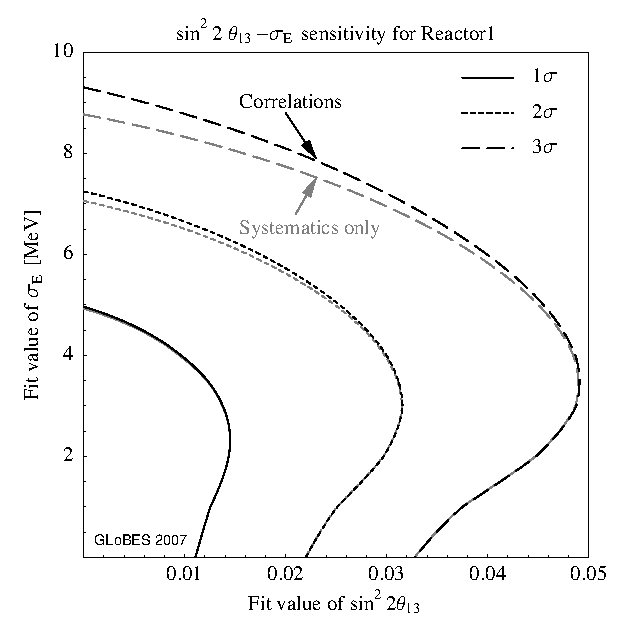
\includegraphics[width=6cm]{reactorNSI}}
\end{center}
}

\section{Using non-standard physics in the application software}

Using more than six parameters in \GLOBES , you will have to maintain the additional parameters. 
For example, there are no standard routines in \GLOBES\ which define projections including more than six parameters, 
which means that you should only use {\tt glbChiNP} further on in order to have a defined behavior
of the projection. In addition, you can still use {\tt glbDefineParams}, but this 
will only access the six standard parameters. You will need to set the additional ones manually using {\tt glbSetOscParams}. 
Do not forget to maintain your non-standard parameters, since any negligence will be punished by un-predicted behavior!

In order to use the non-standard parameters, \GLOBES\ creates any set of oscillation parameters (type {\tt glb\_params})
with the additional parameters. To access the non-standard parameters, you can use the following functions as usual:
\begin{itemize}
\item
\GLB{SetOscParams}
\item
\GLB{GetOscParams}
\item
\GLB{SetProjectionFlag}
\item
\GLB{GetProjectionFlag}
\end{itemize}
In all these cases, the last parameter {\tt which} can now run from $0$ to \GLB{GetNumOfOscParams}{\tt ()-1}. For instance,
\begin{quote}
{\tt
 glbDefineParams(true\_values,0.55,0.15,0.78,0.0,0.000082,0.0022); \\
 glbSetDensityParams(true\_values,1.0,GLB\_ALL); \\
 glbSetOscParams(true\_values,0.0,6);
}
\end{quote}
sets all of the oscillation parameters if you have one additional parameter. 
In addition, the function {\tt glbCopyParams}
can be used to copy all parameters inluding the non-standard ones. For projections,
it is highly recommended not to use any of the {\tt glbChi...} functions anymore except from {\tt glbChiNP},
 in order to have a
predictive behavior of the ``extra'' dimensions.\footnote{It is easy to write headers for new functions
with a self-defined behavior with respect to the new dimensions using {\tt glbChiNP}.} Similar to the oscillation parameters, you can define
the marginalization over the extra parameter(s) by {\tt glbSetProjectionFlag}. You can find a simple
example using non-standard physics with the code from the last section on page~\pageref{ex:nsphysics}.



\chapter{Experimental features$^*$}
\label{chapt:experimental}

Here we describe experimental features currently being implemented in \GLOBES . These features have not yet been tested extensively and should be used with care. They may evolve into standard features in the future, or they may not be supported anymore at a certain point. In general, the number of experimental features is small in a new release version, and increases towards a new version number.

\subsection*{\GLOBES\ 3.0 and higher}

One can change the minimization algorithm in \GLOBES\ with
\begin{function}
\GLBNS{SelectMinimizer}
{\tt int glbSelectMinimizer(int minimizer\_ID)} selects the minimizer \GLBC{GLB\_MIN\_NESTED\_POWELL}, \GLBC{GLB\_MIN\_DEFAULT}, or the hybrid minimizer \GLBC{GLB\_MIN\_POWELL} by the parameter {\tt minimizer\_ID}. 
{\tt GLB\_MIN\_NESTED\_POWELL} is the currently implemented standard algorithm, {\tt GLB\_MIN\_DEFAULT} chooses the standard algorithm at any given time, and {\tt GLB\_MIN\_POWELL} is a faster, yet rarely tested hybrid
minimizer.
\end{function}
Compared to the standard minimization which is performed for systematics first and then for the
oscillation parameters, the hybrid minimizer mixes the systematics and oscillation parameter minimizations. 
This method is much faster,
but correlations between systematics parameters and oscillation parameters might lead to a different convergence behavior in some situations. Thus, when switching to the hybrid minimizer in an application program, one has to reconsider the question whether all degeneracies are found. Since one can change the minimizer at any time, it is recommended that one cross check the minimization for a particular experiment. The danger of modifying the convergence behavior in existing application programs is another reason why the new, faster minimizer is still declared as experimental and not used by default. Note that the meaning of the number of iterations in {\tt glb\_params} changes for the hybrid minimizer. Since the systematics and oscillation parameter minimizations are not strictly separated anymore,  the minimizer does not count the iterations separately, and the total number of iterations is returned. Therefore, it appears that the hybrid minimizer needs more iterations, but, in fact, the default minimizer only counts the oscillation parameter level.


%%% Local Variables: 
%%% mode: latex
%%% TeX-master: Manual.tex
%%% End: 
